\chapter{Annotation Correction and Deformable Models without Landmarks}

% Deformable models are widely used for object detection, localization, recognition and tracking while training a deformable model with good generalisation requires tremendous amount of carefully annotated data, which is extremely time consuming. Even more, annotated data of a specific object category typically requires same numbers of landmarks for every training sample, making the annotation procedure significantly complex where corrext menual annotation of landmarks is impossible in various object classes e.g. ears.

% Despite the fact that that vast majority of existing methods are based on a sparse shape representation, dense shape representation reveals more nuanced structure in terms of [todo: explain].

\begin{figure}[h]
    \centering
        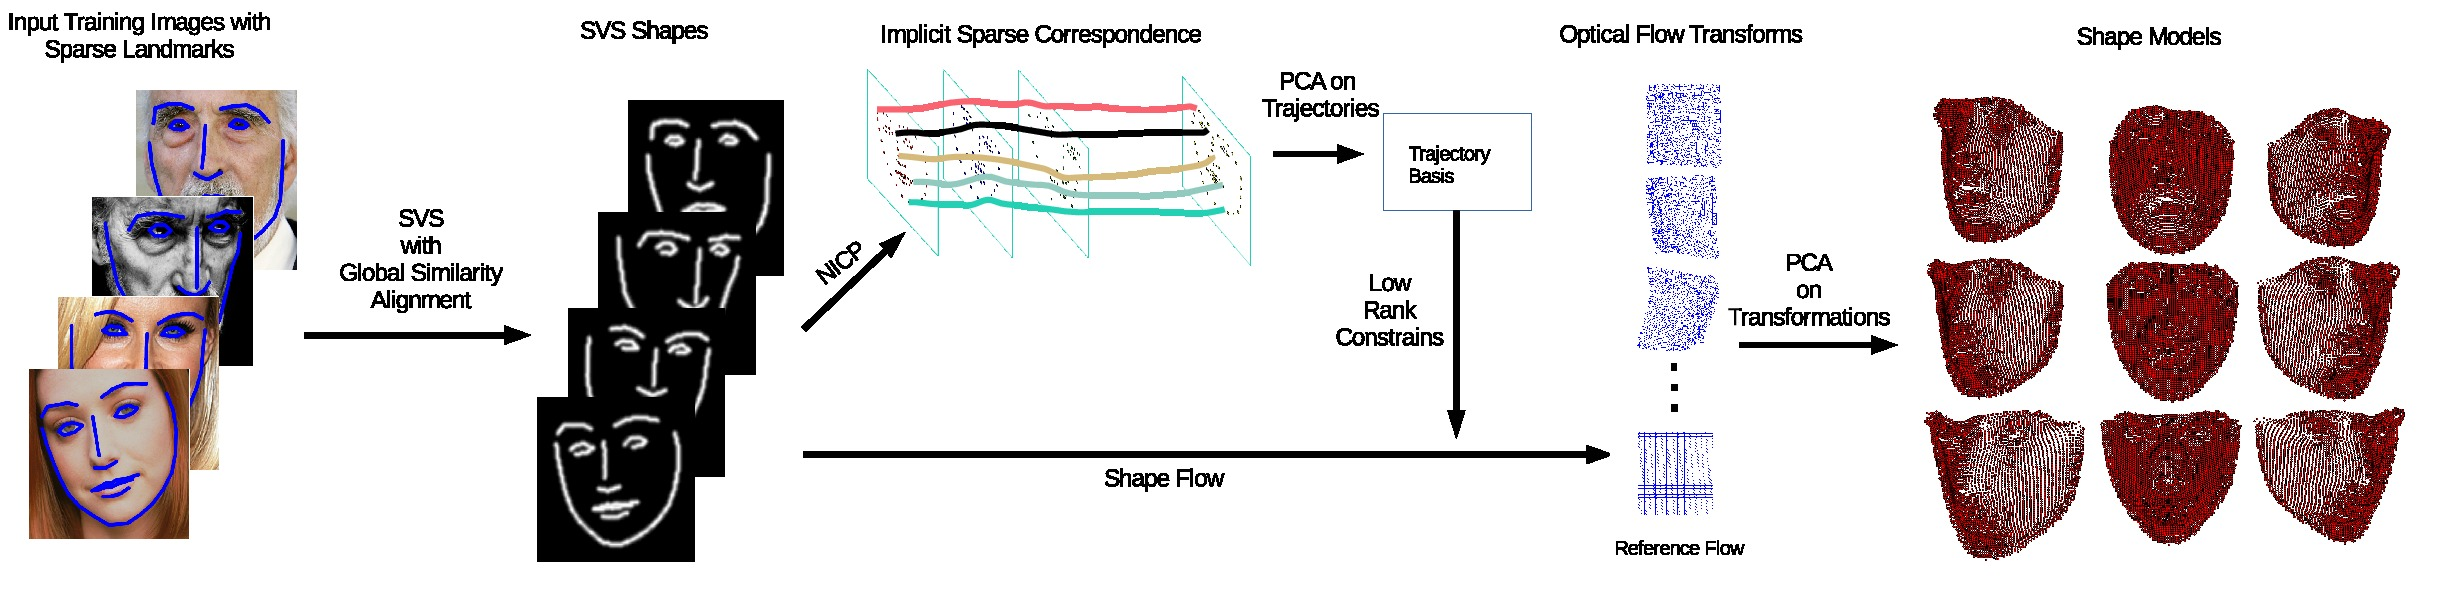
\includegraphics[width=\textwidth]{resources/architecture}
    \caption{Proposed pipeline of constructing dense active appearance model by taking curve annotated training images. The procedure contains following steps: (a) Aligning training images by shapes to remove rotation, translation and scaling information using ICP. (b) Constructing robust shape descriptor using SVS. (c) Building trajectory basis from SVS shapes. (d) Applying shape flow on SVS shapes with low rank trajectory basis. (e) Generating dense shape model by applying PCA on flow transformations.}
    \label{fig:archi}
\end{figure}

We propose a novel framework for building deformable models that does not require any consistent set of annotated landmarks and is based on a dense shape representation. Our method only requires a set of point or curve line annotations that does not need to be consistent over different training samples. It combines the techniques of Non-rigid Iterative Closest Point (NICP) \cite{Amberg2007}, multi-channel Support Vector Shape (SVS) \cite{Nguyen2013} representation and multi-image subspace flow in an effective framework that has significant descriptive power.

The proposed pipeline is depicted in Figure~\ref{fig:archi}. It takes as input a set of training images of a particular object class, along with (possibly inconsistent) point and/or curve line annotations. 
As a first step, the shapes that correspond to the training data are consistently represented using multi-channel SVS. 
The next step is the application of ICP to achieve an initial simple alignment of the SVS images. 
The similarity-aligned SVS images are then fed into a multi-image subspace flow estimation that establishes dense correspondences between all shapes of the training set. In order for the flow estimation to be accurate and exploit the correlation across the different training shapes, it utilises a correspondence basis that is built on sparse correspondences given by Nonrigid ICP alignment of the annotated data. Finally, the dense correspondences that are yielded by the optical flow serve as automatic dense landmarks and are used to define a novel dense version of Active Appearance Models. The following sections discuss the different stages of the proposed pipeline in further detail.

%two major modules. The first module handles inconsistent annotation set by converting to landmark independent shape discriminator. While the other module produces shape flow on object discriminators to generate dense flow transformations in shape space following by robust PCA\cite{?} to generate deformable model. In this section, we present the entire architectures, design decision and algorithms.
\section{Shape Representation Without Consistent Annotations}
\label{sec:svs}
%Ordinarily, construction of deformable model requires training data set having consistent number of landmarks. But unavoidable changes has to be made before applying same algorithm on diverse annotated data set.

In order to fully capture the variability among most deformable object shapes annotations, we use a representation based on Support Vector Shapes (SVS) \cite{Nguyen2013}. As described in section \ref{sec:bg_svs}, an SVS is a decision function trained on shapes using Support Vector Machines (SVMs) with  Radial Basis Function (RBF) kernels. In this way, a shape is represented as a classifier function, which has several advantages: (a) The representation is completely general, \eg it can be applied to sparse landmark points, curves lines or a combination of the two and (b) It fuses inconsistent landmarks into consistent and directly comparable decision functions. Furthermore, this representations is also robust against noise, missing data and outliers.

In practice, we assume that all the training images correspond to the same object category and contain a set of inconsistent points and curve line annotations. All annotations are densely sampled to yield a set of annotated landmarks per image, with this set being different for every training image. Initially, negative points get randomly sampled around sparse landmarks while annotated landmarks are positive points. Since the number of positive points is far smaller that the number of negative ones, landmarks are assigned considerably larger weights so that $N_p \times W_p=N_n \times W_n$ where $N_p, N_n$ are number of positive/negative samples and $W_p, W_n$ are their corresponding weights.

SVMs with RBF kernel function map any numbers of data points onto an infinite-dimensional space where positive and negative points are linearly separable, hence the classification boundary on 2D space represents the actual shape of the object. Note that the decision function for SVMs can be mathematically expressed as:
\begin{equation} \label{eq:decisionfunc}
    d(\mathbf{x})=\sum_i\alpha_i \, k(\mathbf{x}_i^*,\mathbf{x})
\end{equation}
where $\mathbf{x}_i^*$ are support vectors and \mbox{$k(\mathbf{x}_i^*, \mathbf{x}) = exp(-\lambda \|\mathbf{x}_i^* -\mathbf{x}\|^2)$} is the RBF kernel .

Figure \ref{fig:build_svs} shows an exemplar shape representation using SVS. As it can be observed, the final result does not drastically depend on the original number of annotated landmarks.


\begin{figure}[h]
    \centering
    \begin{subfigure}[b]{0.4\textwidth}
            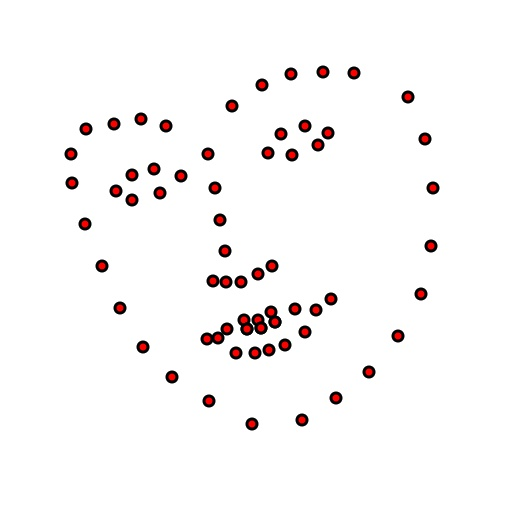
\includegraphics[width=\textwidth]{resources/landmark}
        \caption{Spare landmarks}
    \end{subfigure}
    \hfill
    \begin{subfigure}[b]{0.4\textwidth}
            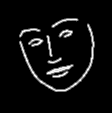
\includegraphics[width=\textwidth]{resources/svs}
        \caption{Decision function}
        \label{fig:svs}
    \end{subfigure}
    \caption{Exemplar SVS shape representation. The decision function is trained on the set of sparse landmarks. In (b), brighter colour represents higher probability of a pixels belonging to the original shape.}
    \label{fig:build_svs}
\end{figure}


After constructing the SVS representation for all images, the next step is to apply a simple similarity alignment over them. This is done because the goal here is to build a model capable of effectively representing non-rigid local shape deformations rather than global rotation, translation and scaling. The alignment is performed by using the Iterative Closest Point (ICP) algorithm \cite{Besl1992} on the annotated landmarks point cloud of the training images. Algorithm details can be found in section \ref{sec:bg_icp}.


\section{Shape Correspondence Basis}

In order to robustly establish dense correspondences across all SVS images using optical flow, it is important to constrain how pixels are allowed to move from one SVS image to another. In this work, we constrained the range of allowed pixels movements by learning a correspondence subspace. 

In order to learn the such a subspace, we first transform the original annotation to point clouds. Then, we use Nonrigid Iterative Closest Point (NICP) to align the previous point clouds with respect to a reference point cloud template. NICP iteratively deforms each point cloud until its points match the ones on the shape template and sparse correspondences are established. However, because optical flow is a pixel-wise frame registration technique, we need to establish correspondences for all pixels on the reference frame rather than for sparse point clouds. To achieve this, we apply Thin Plate Spline (TPS) \cite{Bookstein1989} to interpolate intermediate points to find correspondences for all pixels in the reference frame given the point cloud correspondences provided by the previous NICP stage. Once dense correspondences have been established among all pixels, the so-called correspondence subspace is obtained by performing PCA on the trajectory of all pixels. Note that incorporating the previous subspace as a low rank constrained in optical flow is consistent with its assumption of smooth motion.


% ---------------------------------------------------------------------------------------------------------------------------------------------------


\section{Shape Flow}
\label{sec:shapeflow}

Using the SVS functions built from training data, the next step of our pipeline is to establish dense correspondences between all these functions. We propose to do this procedure jointly, by using the correspondence basis. This procedure shares similarities with multi-frame optical flow and we call it Shape flow. We build upon robust methods for  optical flow estimation. Optical flow estimation typically works based on the assumptions of brightness or colour constancy and motion smoothness. However, in terms of shapes, neither constant illumination nor continuous motion exists in sequence of shapes as all training data are independent. 
For this reason, we propose to modify the formulation of multi-frame optical flow by using the correspondence basis that we introduced in conjunction with the SVS functions, rather than actual images.

\subsection{Non-rigid ICP and Correspondence Basis Creation} \label{sec:trabasis}
Since shapes from training data set having completely no motion smoothness, it is of importance to contain constrains in optimization on translation of pixels from one shape frame to another. We constrain the optimization on trajectory subspace.
We supervise trajectories from sparse landmarks. To begin with, Non-rigid Iterative Closest Point (NICP)\cite{Amberg2007} applied on sparse annotated points and/or lines. NICP deforms source points to fit template iteratively until convergence, thereby all points on source deformed to establish one-to-one points correspondence with template. Performing the algorithm for all training shapes will get an implicit point correlation between sparse shapes.

Since optical flow pixel-wise frame registration, the trajectory basis build should also match the dimension, which is dense on shapes with trajectory length depends on number of training data. With correspondences produced after applying NICP, Thin-Plate Spline (TPS)\cite{Bookstein1989} transformations are utilized to warp every shape planes to template plane thereby generates an implicit dense shape registering. For all dense transformations $\bm{u_n}(\bm{x}), n \in \{1,...,F\}$, where $F$ is number of data and $\bm{x}$ is vector of pixels, Principle Component Analysis (PCA) is performed on trajectory to obtain low rank trajectory basis:
\begin{equation}
    \begin{bmatrix}
        \bm{u_1}(\bm{x}) \\
        \vdots \\
        \bm{u_F}(\bm{x})
    \end{bmatrix}
    =
    \begin{bmatrix}
        \bm{q_1}(1) & \cdots & \bm{q_R}(1) \\
        \vdots      & \ddots & \vdots  \\
        \bm{q_1}(F) & \cdots & \bm{q_R}(F)
    \end{bmatrix}
    \times
    \begin{bmatrix}
        \bm{v_1}(x) \\
        \vdots \\
        \bm{v_R}(x)
    \end{bmatrix}
\end{equation}
where $\bm{q_i}(n)$ are low rank components with $R \ll 2F$ and $\bm{v_i}(x)$ weighted each component with dependencies on $x$. Simpler expression shown below:
\begin{equation}
    \bm{u_n}(\bm{x})=\sum_{i=1}^R\bm{q_i}(n)\bm{v_i}(x)+\bm{\varepsilon_n}(\bm{x})
\end{equation}
Although optical flow on shapes made under the assumption that objects motion are smooth, the low rank constrain on trajectory basis recovered the hypothesis. Section \ref{exp:basis} investigate the impact of introducing subspace constrains for shape flow. 

\subsection{Multi-image Subspace Flow}
To register all decision functions to template shape, decision function $d_i(\bm{x}), i \in {1,...,F}$ are grouped into one sequence before applying flow algorithm. The objective cost function we would like to minimise is:
\begin{align}
    \operatorname*{arg\,min}_{\bm{u_n}(\bm{x}), \bm{v}}&=\alpha \int_{\Omega}\sum_{n=1}^F|\bm{d_n}(x+\bm{u_n}(x))-\bm{d_0}(x)\| dx  \label{eq:costfunc}\\
    &+ \beta \int_{\Omega}\sum_{n=1}^F\|\bm{u_n}(x)-\sum_{i=1}^R\bm{q_i}(n)\bm{v_i}(x)\|^2 dx \label{eq:lowrank}\\
    &+ \sum[\bm{TV}(Qv)]
\end{align}
where $d_n(x)$ is the decision function from~\eqref{eq:decisionfunc}, which returns possibilities of given coordinate classified as shape component where coordinates are from set $\Omega \in \Re^2$. $TV(Qv)$ is total variation as regularization on low rank subspace, $Q$ is trajectory basis and $v^T.L.v$ is low rank spacial constrains.

Term~\eqref{eq:costfunc} state the shape constancy where points having similar classification probability are from same object.
Part~\eqref{eq:lowrank} applies constrain on low rank trajectory basis states in section~\ref{sec:trabasis}.
The objective cost function has two free parameters $u$ and $v$, so we perform alternating minimisation. The equation can be solved using a thresholding scheme after linearisation of image functions. The minimisation can be speed up by paralleling the minimisation for every spatial-temporal point $(x;n), x \in \Omega, n \in \{1,...F\}$ independently.

As a result of solving the equation, $\bm{u_n}(\bm{x}), x \in \Omega$ gives a group of deformation fields that registering every decision functions in the shape sequence to reference frame e.g. $\bm{u_1}(\bm{x})$ registers decision function $\bm{d_1}(\bm{x})$ to the reference frame. Figure~\ref{fig:deformationfield} demonstrates deformation fields that warps from reference frame where there is no deformation.

\begin{figure}[h]
    \centering
    \begin{subfigure}[b]{0.15\textwidth}
            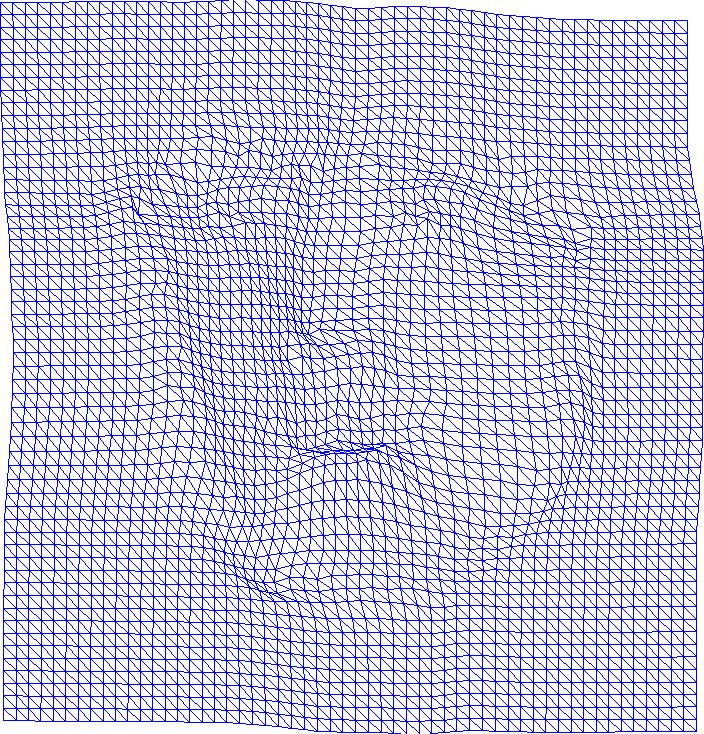
\includegraphics[width=\textwidth]{resources/Fig_Flows/0}
    \end{subfigure}
    \hfill
    \begin{subfigure}[b]{0.15\textwidth}
            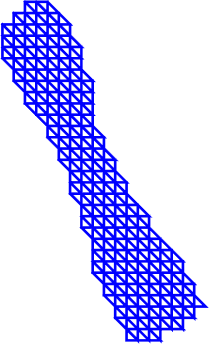
\includegraphics[width=\textwidth]{resources/Fig_Flows/1}
    \end{subfigure}
    \hfill
    \begin{subfigure}[b]{0.15\textwidth}
            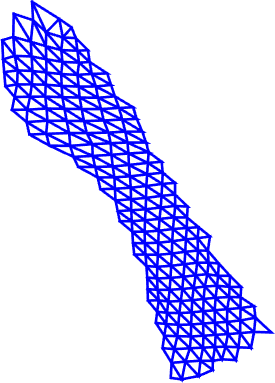
\includegraphics[width=\textwidth]{resources/Fig_Flows/2}
    \end{subfigure}
    \\
    \begin{subfigure}[b]{0.15\textwidth}
            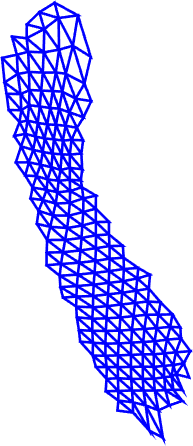
\includegraphics[width=\textwidth]{resources/Fig_Flows/3}
    \end{subfigure}
    \hfill
    \begin{subfigure}[b]{0.15\textwidth}
            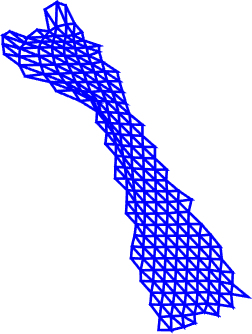
\includegraphics[width=\textwidth]{resources/Fig_Flows/4}
    \end{subfigure}
    \hfill
    \begin{subfigure}[b]{0.15\textwidth}
            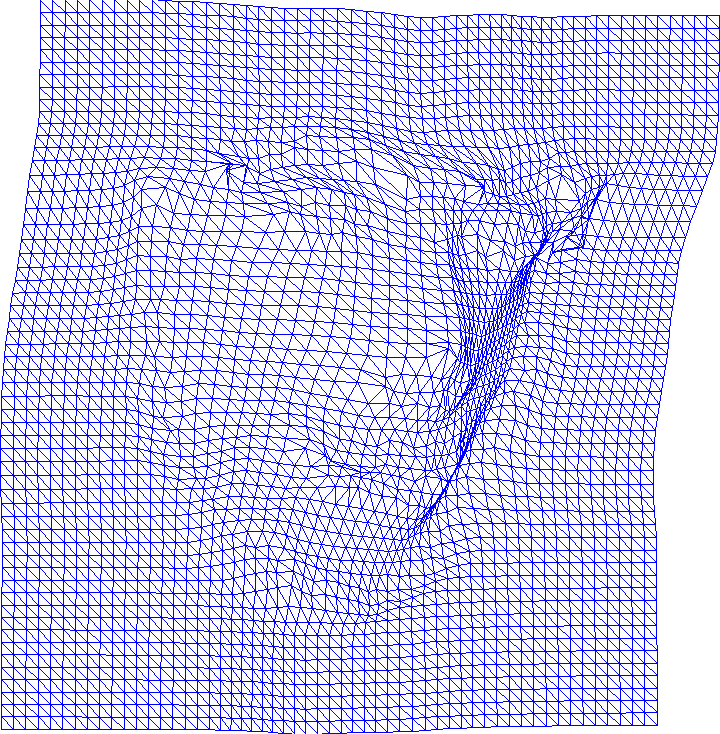
\includegraphics[width=\textwidth]{resources/Fig_Flows/5}
    \end{subfigure}
    \\
    \begin{subfigure}[b]{0.15\textwidth}
            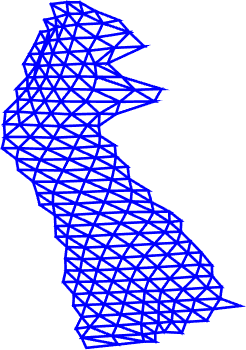
\includegraphics[width=\textwidth]{resources/Fig_Flows/6}
    \end{subfigure}
    \hfill
    \begin{subfigure}[b]{0.15\textwidth}
            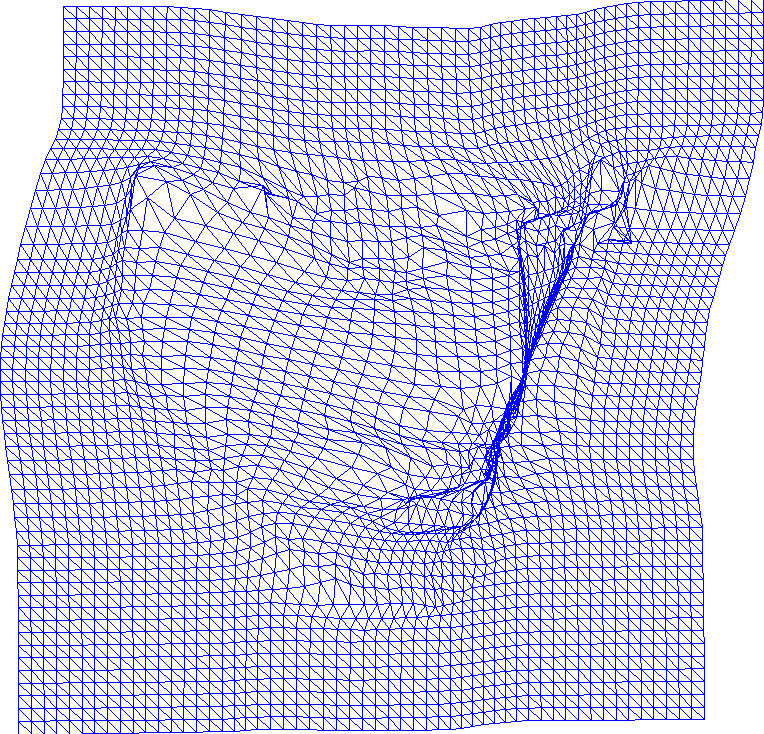
\includegraphics[width=\textwidth]{resources/Fig_Flows/7}
    \end{subfigure}
    \hfill
    \begin{subfigure}[b]{0.15\textwidth}
            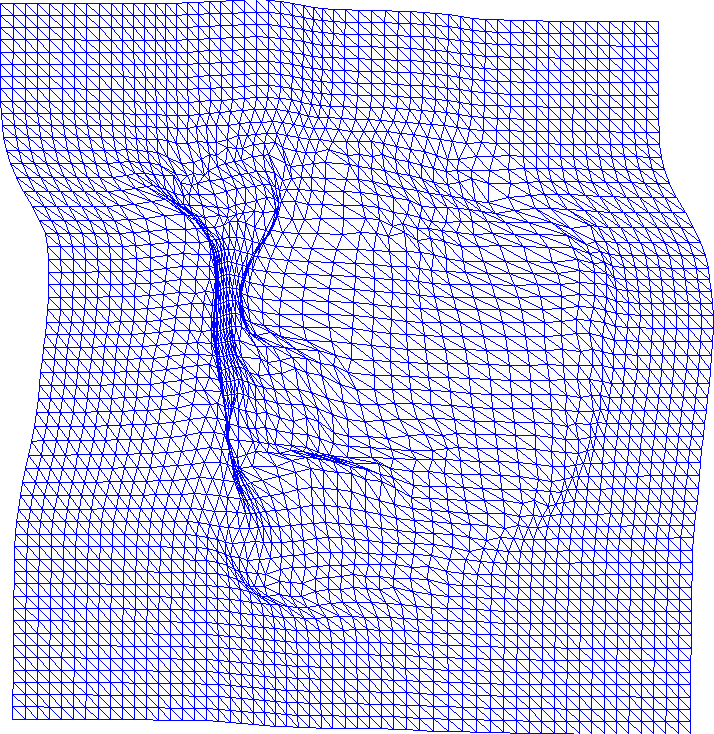
\includegraphics[width=\textwidth]{resources/Fig_Flows/8}
    \end{subfigure}
    \caption{Deformation field built from shape flow. Each subplot represents a transformation to register given image to reference frame, where the deformation field to register reference frame to itself is non-deformed grid.}
    \label{fig:deformationfield}
\end{figure}


Applying PCA on deformations trains dense deformable shape model:
\begin{equation*}
    \bm{s_p}=\bm{\bar{s}} + \bm{U}_s\bm{p}
\end{equation*}
where $\bm{s_p}$ is deformed shape instance. $\bm{\bar{s}}$ is mean shape and $\bm{U}_s\bm{p}$ are eigenvectors with corresponding parameters $p$. Figure~\ref{fig:models} shows an instance of deformed shape and appearance model.
\begin{figure}[h!]
    \centering
    \begin{subfigure}[b]{0.4\textwidth}
            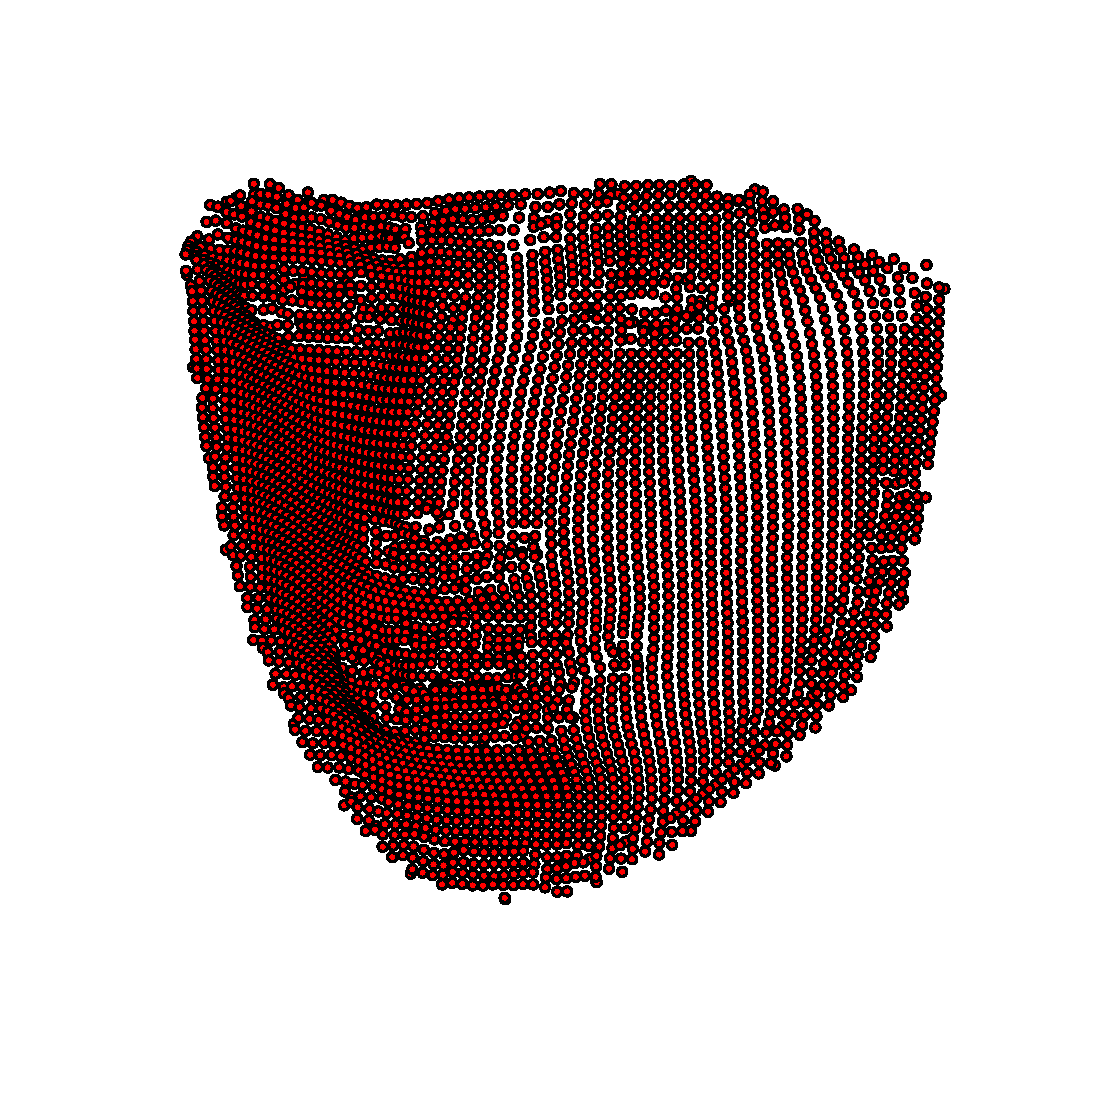
\includegraphics[width=\textwidth]{resources/Fig_dAAM/of_shape}
    \end{subfigure}
  	\hfill
    \begin{subfigure}[b]{0.4\textwidth}
            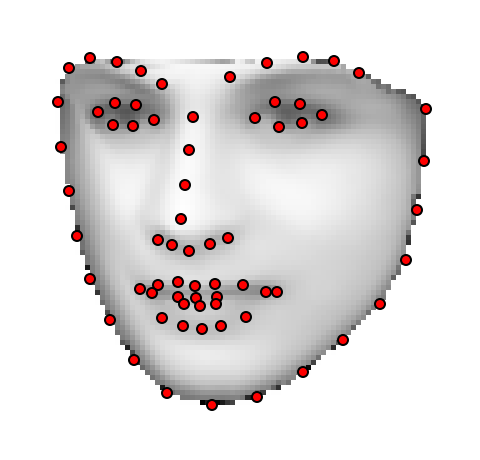
\includegraphics[width=\textwidth]{resources/Fig_dAAM/of_app}
    \end{subfigure}
    \caption{Dense Deformable Model}
    \label{fig:models}
\end{figure}

% \begin{figure}[h!]
%     \centering
%     \begin{subfigure}[b]{0.22\textwidth}
%             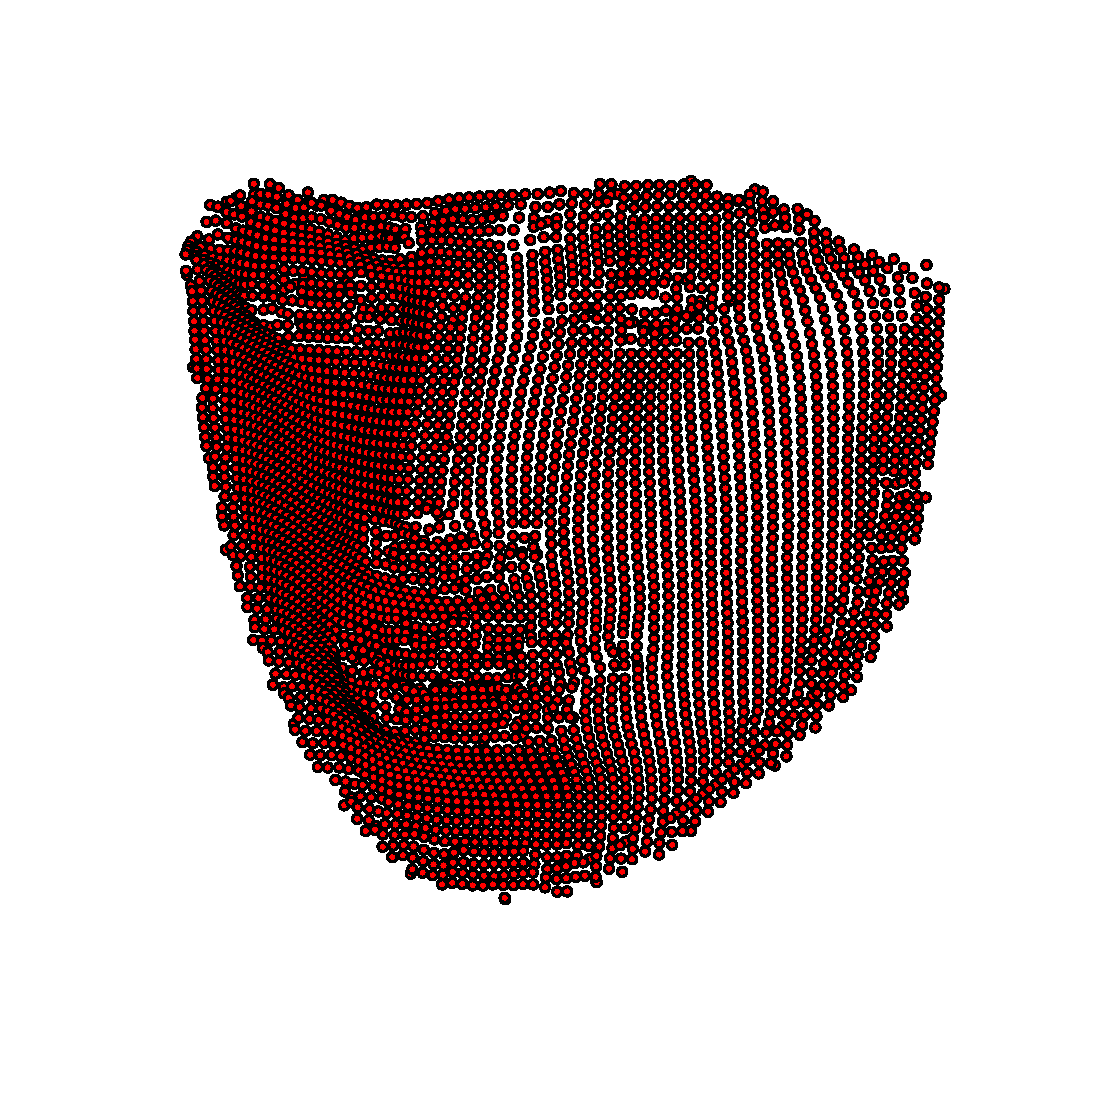
\includegraphics[width=\textwidth]{resources/Fig_dAAM/of_shape}
%     \end{subfigure}
%   	\hfill
%     \begin{subfigure}[b]{0.22\textwidth}
%             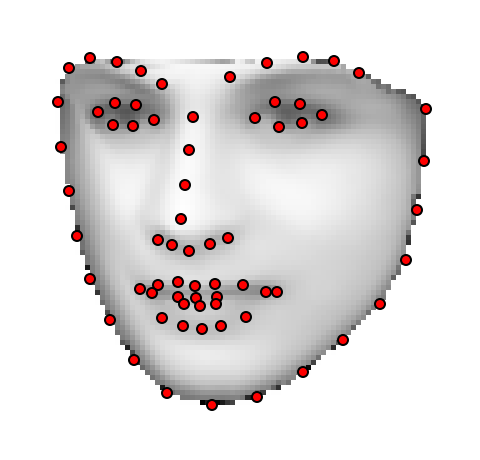
\includegraphics[width=\textwidth]{resources/Fig_dAAM/of_app}
%     \end{subfigure}
%     \caption{Dense Deformable Model}
%     \label{fig:models}
% \end{figure}

\section{Dense Active Appearance Models}

The deformation fields obtained in section \ref{sec:shapeflow} can be effectively used to learn a naturally dense version of Active Appearance Models \cite{Cootes2001, Matthews2004}. Because all deformation fields contain the same number of pixels (the same as on the reference frame) the spatial positions $\mathbf{x}_i=(x_i, y_i)$ of these pixels can be treated as point landmarks and the deformation field themselves as dense annotations of the object's shape. Consequently, building a dense shape model reduces to normalizing these dense annotations with respect to a global similarity transform (typically using Procrustes Analysis) and applying Principal Component Analysis (PCA). The resulting shape model can be mathematically expressed as:
\begin{equation}
    \begin{aligned}
        \mathbf{s} & = \mathbf{\bar{s}} + \mathbf{S} \mathbf{p}
    \end{aligned}
    \label{eq:shape_model}
\end{equation}
where $\mathbf{\bar{s}}$ is mean shape and $\mathbf{S}$ and $\mathbf{p}$ are the shape bases and parameters respectively.

On the other hand, the texture model associated to the previous set of densified shapes can be easily obtained by warping all image onto the reference frame, making explicit use of the one-to-one correspondence between pixels on the reference frame and on the deformation fields. Once the images have been warped, the texture model is obtained by applying PCA on the warped images. The texture model is mathematically defined by the following expression:
\begin{equation}
    \begin{aligned}
        \mathbf{a} = \mathbf{\bar{a}} + \mathbf{A} \mathbf{c}
    \end{aligned}
	\label{eq:tex_model}
\end{equation}
where $\mathbf{\bar{a}}$ is the mean texture, and $\mathbf{A}$ and $\mathbf{c}$ are the texture bases and parameters respectively.

Note that, both shape and texture models are directly related through the existent one-to-one correspondence between dense landmarks and pixels on the reference frame. Therefore, in clear contrast to classic AAMs formulations \cite{Cootes2001, Matthews2004}, no motion model (piece-wise affine, thin-plates splines \cite{Bookstein1989}) is required to relate the previous shape and texture models in our dense formulation. As noted by other authors \cite{Amberg2009, Tzimiropoulos2014}, this has the advantage that all efficient compositional gradient descent algorithms for fitting AAMs \cite{Papandreou2008, Matthews2004, Amberg2009, Tzimiropoulos2013, Alabort2014} become exact under our formulation. 

%\subsection{Drawing Annotation}
%The purpose of the shape descriptor $\bm{d_i}(x)$ generates probabilities for arbitrary points. If we sample points that are exactly pixel-wise integers, and normalise classification value, we can visualise a SVS as an image for example in figure~\ref{fig:svs}. In other words, our architecture will also works for images with landmarks similar to SVS visualisations like drawing. Assuming the intensity of a gray-scale image simulate the decision function, named $\bm{I_i}(x), x \in \Omega, i \in \{1,...F\}$. But in this situation, pixels at image space are discontinued, so $x$ is constrained to be integer and within the view window of size $N\times M$.


\chapter{Evaluation}

This sections evaluates the performance of dense Active Appearance Models (dAAMs) built using the proposed methodology in the problem of non-rigid object alignment in-the-wild. Results for four different experiments are reported. Experiments \ref{exp:svs} and \ref{exp:basis} investigate the impact that the Support Vector Shape representation and the subspace constrains for shape flow have, respectively, on the fitting accuracy achieved by dense AAMs build using the proposed pipeline. Experiments \ref{exp:face} and \ref{exp:ear} compare the fitting accuracy of our dense AAMs with respect to that of classic AAMs on the problems of non-rigid face and ear alignment in-the-wild. 
% Finally, experiment \ref{exp:lose} evaluates the effectiveness and performance of the proposed methodology to build dense AAMs of objects that are difficult to annotated with respect to a consistent set of landmarks, such as bottles and human bodies. 
Note that all results reported in this section were obtained by fitting all AAM (dense and classic) using the fast version of the Simultaneous Inverse Compositional algorithm (Fast-SIC) originally proposed by the authors of \cite{Papandreou2008}. For further experimental results and visualizations please refer to our supplementary material. 

%In this section we evaluate the performance of the proposed methodology in a variety of tasks. Results for 4 different experiments are reported. Experiment \ref{exp:1} compares the fitting accuracy of Dense Active Appearance Models (DAAMs) built using our methodology with respect to that of classic AAMs on the problems of non-rigid face and ear alignment in-the-wild. Experiment \ref{exp:2} investigates the impact that the Support Vector Shape representation has on the performance achieved by DAAMs on the the first experiment. Experiment \ref{exp:3} evaluates the effectiveness of the proposed methodology to build DAAMs of objects that are difficult to annotated with respect to a consistent set of landmarks, such as bottles and human bodies. Finally, experiment \ref{exp:4} serves as a qualitative demonstration of how the proposed pipeline can use be effectively used to generate novel modified instances of an object, e.g. caricatures, from simple hand drawn sketches


\section{Shape Representation}
\label{exp:svs}

This experiment investigates the impact that the SVS representation described in section \ref{sec:svs} has on the final fitting accuracy achieved by dense models built using the propose pipeline. In particular, we compare the SVS representation with a simpler shape representation that consists of directly using binary images obtained from curve line annotations. In order to make the experiment fair we keep all remaining stages of the pipeline intact and simply change between these two shape representations. We use our methodology to build two dense AAMs, one using the SVS representation (SVS-dAAMs) and another using the binary shape representation (Binary-dAAMs). Both models were built using 811 training images of the Labelled Faces Parts in-the-Wild (LFPW) \cite{Belhumeur2011} database and tested on 224 testing images of the same database. We re-annotated all images from this database using the proposed curve line annotation scheme. In order to provide quantitative results, we annotated the reference frame of both dense AAMs (2 images) with the standard 68 point annotation scheme provided by the iBUG group\footnote{\label{ibug_300} \url{http://ibug.doc.ic.ac.uk/resources/300-W/}}. Note that, any set of landmarks annotated on the reference frame can be easily extrapolated to any shape generated by dense shape models.
%; for example, by interpolating its relative position with respect to its immediate reference frame neighbours on the newly generated dense shape instance, \ref{fig:extrapolate_landmarks}. 
Accuracy is reported in terms of the normalized point-to-point error measure described in \cite{Zhu2012}.

The Cumulative Error Distribution (CED) for this experiment is shown in Figure \ref{fig:svs_ced} while fitting statistics are reported in Table \ref{tab:svs_stats}. Looking at the results it can be clearly seen that using SVS results in a constant $\approx$5\% improvement over the simple binary shape representation for almost all CED graph and on the reported fitting statistics.

\begin{figure}[h]
\centering
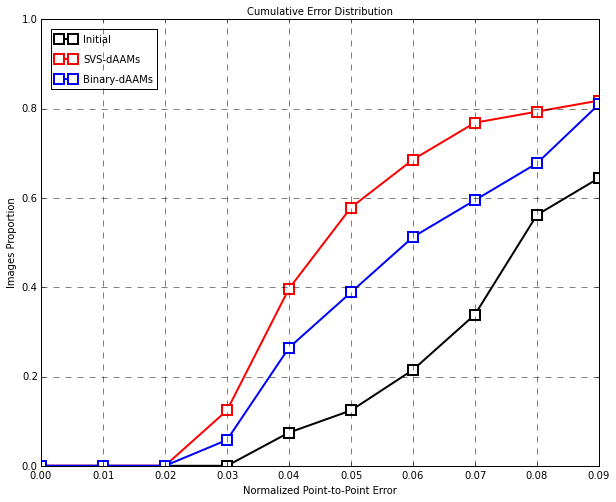
\includegraphics[width=0.7\textwidth]{resources/Fig_SVS/svs_ced}
\caption{CED over 68 landmarks on the LFPW database for experiment \ref{exp:svs}}
\label{fig:svs_ced}
\end{figure}

\begin{table}[h]
\small
\centering
\begin{tabular}{|l|c|c|c|}
\hline
\emph{Method}       & \emph{mean $\pm$ std} & \emph{median} & $\leq 0.05$\\
\hline\hline
Initialization      & 0.0805 $\pm$ 0.0246 & 0.0785 & 12\%\\
SVS                 & 0.0583 $\pm$ 0.0297 & 0.0443 & 57\%\\
Binary              & 0.0640 $\pm$ 0.0300 & 0.0588 & 39\%\\
\hline
\end{tabular}
\caption{Fitting statistics on the LFPW database for experiment \ref{exp:svs}}
\label{tab:svs_stats}
\end{table}

\section{Constrained Basis}
\label{exp:basis}

This experiment investigate the impact of introducing subspace constrains for shape flow. The shape representations of training data are independence, thus simply applying flows on shapes breaks the fundamental assumption of motion smoothness. The hypothesis is able to be maintained for shapes as described in section~\ref{sec:trabasis}. To be specific, we take measures of point-to-point error for fitting same data with our pipeline with same configuration, but only alter the low rank basis. 

The experiment results are manifested by constructing two dense AAMs, Basis-dAAMs and no-Basis-dAAMs,among 811 training images from Labelled Faces Parts in-the-Wild (LFPW)\cite{Belhumeur2011} database with 224 testing images using same annotation scheme by iBUG\footnoteref{ibug_300}. 
Cumulative error distributions are shown in Figure~\ref{fig:basis_ced} and corresponding statistics are listed in Table~\ref{tab:basis_stats}. 
It shows shape flow with constrained basis outperforms, constantly, standard flow technique by an unavoidable amount, which significantly supported the necessities of our low rank basis introduced in~\ref{sec:trabasis}.

\begin{figure}[h]
\centering
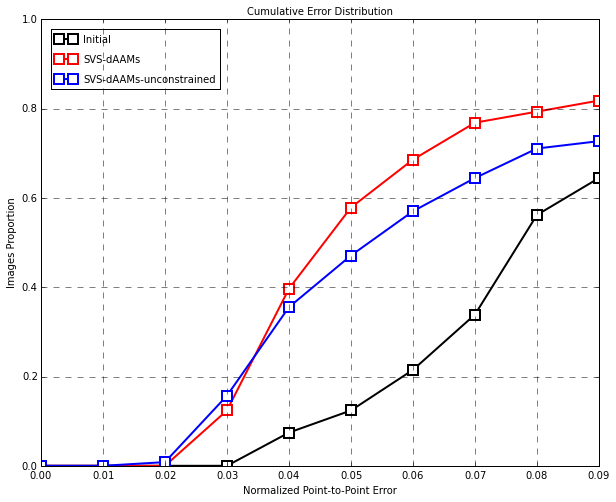
\includegraphics[width=0.7\textwidth]{resources/basis_ced}
\caption{CED over 68 landmarks on the LFPW database for experiment \ref{exp:basis}}
\label{fig:basis_ced}
\end{figure}

\begin{table}[h]
\small
\centering
\begin{tabular}{|l|c|c|c|}
\hline
\emph{Method}       & \emph{mean $\pm$ std} & \emph{median} & $\leq 0.05$\\
\hline\hline
Initialization      & 0.0805 $\pm$ 0.0246 & 0.0785 & 12\%\\
Constrained Flow    & 0.0583 $\pm$ 0.0332 & 0.0443 & 57\%\\
Unconstrained Flow  & 0.0698 $\pm$ 0.0458 & 0.0556 & 46\%\\
\hline
\end{tabular}
\caption{Fitting statistics on the LFPW database for experiment \ref{exp:basis}}
\label{tab:basis_stats}
\end{table}



\section{Non-rigid object alignment in-the-wild}
\label{exp:alignment}

In the following set of experiments we use the proposed methodology to build dense AAMs of various object classes (faces, ears, bottles and body pose) and quantitatively asses their respective fitting accuracy when fitted to novel in-the-wild images of the previous objects.

\subsection{Face alignment}
\label{exp:face}

This experiment compares the fitting accuracy of our dense AAM versus the one of classic AAM on the problem of non-rigid face alignment in-the-wild. For this experiment, both models were built using the 811 training images of the Labelled Faces Parts in-the-Wild (LFPW) \cite{Belhumeur2011} database. Classic AAM were built from 68 point landmark annotations\footnoteref{ibug_300} using the standard procedure described in \cite{Cootes2001, Matthews2004}; piece-wise affine was used as their motion model. Our dense AAM were built as described in experiment \ref{exp:svs}. Given the evidence obtained from that experiment, we used SVS as the shape representation used throughout our pipeline.

Results for this experiment are reported over the 224 testing images of the LFPW database using again 68 point ground truth landmark annotations\footnoteref{ibug_300}. For this experiment, we report results using two different image representations, \ie pixels intensities (INT) and Histogram of Oriented Gradients (HOG) \cite{Dalal2005} for both models. The two techniques were initialized using our own version of the face detector described in \cite{Zhu2012}.

Cumulative Error Distributions (CED) for this experiment are shown in Figure \ref{fig:face_ced} while fitting statistics are reported in Table \ref{tab:face_stats}. Results show that, for this experiment, the fitting accuracy achieved by our dense AAM is comparable to the one achieved by classic AAMs using both image representations. In particular, our method seems to perform marginally better when pixel intensities are used as the image representation, while classic AAMs slightly outperform our technique for HOG. Overall, both methods achieve similar performance for errors below 5\%. We believe this results are remarkable, provided that our model was learned from curve annotations ($\approx$ 30 seconds/image) instead of expensive point landmark annotations ($\approx$ 4 minutes/image).

\begin{figure}[h]
\centering
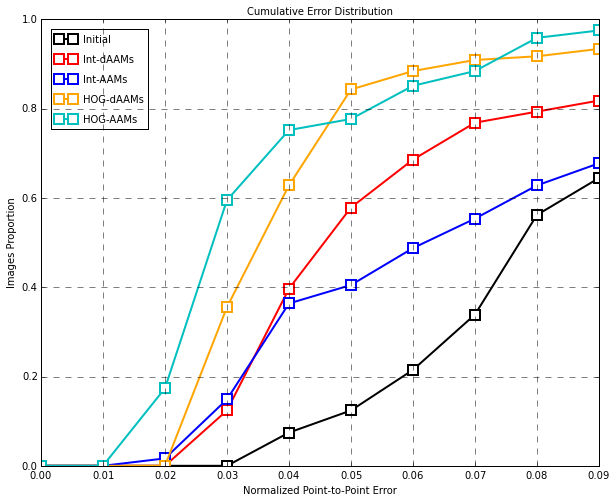
\includegraphics[width=0.7\textwidth]{resources/Fig_Alignment/face_ced}
\caption{CED over 68 landmarks on the LFPW database for experiment \ref{exp:face}}
\label{fig:face_ced}
\end{figure}

\begin{table}[h]
\small
\centering
\begin{tabular}{|l|c|c|c|}
\hline
\emph{Method}   & \emph{mean $\pm$ std} & \emph{median} & $\leq 0.05$\\
\hline\hline
Initialization  & 0.0805 $\pm$ 0.0246 & 0.0785 & 12\%\\
INT - dAAM      & 0.0583 $\pm$ 0.0332 & 0.0443 & 57\%\\
INT - AAM       & 0.0876 $\pm$ 0.0608 & 0.0797 & 40\%\\
HOG - dAAM      & 0.0413 $\pm$ 0.0212 & 0.0340 & 85\%\\
HOG - AAM       & 0.0354 $\pm$ 0.0210 & 0.0266 & 77\%\\
\hline
\end{tabular}
\caption{Fitting statistics on the LFPW database for experiment \ref{exp:face}}
\label{tab:face_stats}
\end{table}

\subsection{Ear alignment}
\label{exp:ear}

In this experiment, we studied the feasibility of building and fitting statistical deformable models that capture the variability of the human ear. To this end, we collected 605 high resolution images of ears in unconstrained scenarios and annotated them using both a newly defined 55 point annotation scheme for ears and the curve annotations proposed in this report. Examples of these two type of ear annotations are shown in Figure \ref{fig:intro}. We randomly split the previous database into two disjoint sets of training (500) and testing (105) images. We compare the fitting accuracy obtained by our dense AAM model versus the one of classic AAM on these data. Both models were built using the 500 images on the previous training set and their fitting accuracy evaluated on the 105 images of the testing set. Note here that we used the same procedures used in experiment \ref{exp:svs} to build the models and evaluate the results (piece-wise affine motion model for classic AAM and SVS, constrained flow and landmark interpolation for dense AAM).

\begin{figure}[h]
\centering
    \begin{subfigure}[b]{0.23\textwidth}
            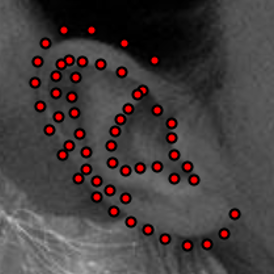
\includegraphics[height=1\textwidth]{resources/Fig_Alignment/ear_06_55}
    \caption{$0.06$}
    \end{subfigure}
    \begin{subfigure}[b]{0.23\textwidth}
            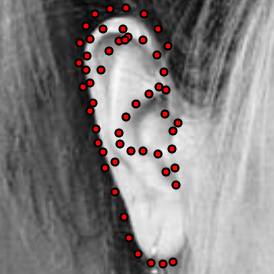
\includegraphics[height=1\textwidth]{resources/Fig_Alignment/ear_1_55}
    \caption{$0.1$}
    \end{subfigure}
    \begin{subfigure}[b]{0.23\textwidth}
            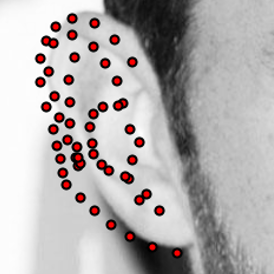
\includegraphics[height=1\textwidth]{resources/Fig_Alignment/ear_14_55}
    \caption{$0.14$}
    \end{subfigure}
    \begin{subfigure}[b]{0.23\textwidth}
            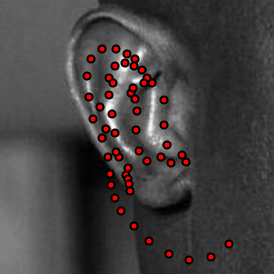
\includegraphics[height=1\textwidth]{resources/Fig_Alignment/ear_23_55}
    \caption{$0.23$}
    \end{subfigure}
\caption{Qualitative examples showing different values of normalize point-to-point error measure for ears.}
\label{fig:ear_error}
\end{figure}

Results for this experiments are shown in Figure \ref{fig:ear_ced} and Table \ref{tab:ear_stats}. In this case, we can readily observe that the accuracy achieved by ear models, in terms of the previous normalized point-to-point error measure, is lower than the one achieved by face models. This result is expected due to the more complex structure of the ear shape. Through visual inspection we determined that fitting errors below $0.1$ for ears typically look plausible under the previous error measure \ref{fig:ear_error}. Results for this experiment show that our approach performs significantly better than the classic AAM when pixels intensities are used as image representation. In fact, classic AAM fail to improve the accuracy of the original initialization on $\approx45\%$ of the test images while for our the case of our dense model this number goes up to $\approx70\%$. On the other hand, the accuracy of both models dramatically improves using HOG. In this case, classic AAM outperform our dense AAM for small errors up to $0.1$ while both models obtain similar results for errors around $0.1$. Again, the fact that the propose pipeline is capable of dealing with the complex structure of the ear shape and learn dense AAM from simple curve line annotations that can compete and even surpass (in the case of a simple pixel intensity image representation) classic AAM, build from carefully annotated point landmarks, is quite remarkable. 

\begin{figure}[h]
\centering
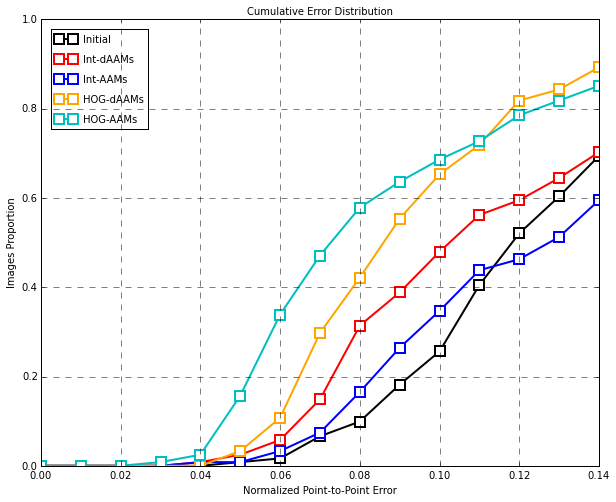
\includegraphics[width=0.7\textwidth]{resources/Fig_Alignment/ear_ced}
\caption{CED over 55 landmarks on the collected ear database for experiment \ref{exp:ear}}
\label{fig:ear_ced}
\end{figure}

\begin{table}[h]
\small
\centering
\begin{tabular}{|l|c|c|c|}
\hline
\emph{Method}   & \emph{mean $\pm$ std} & \emph{median} & $\leq 0.1$\\
\hline\hline
Initialization  & 0.1246 $\pm$ 0.0394 & 0.1186 & 32\%\\
INT - dAAM      & 0.1180 $\pm$ 0.0533 & 0.1030 & 47\%\\
INT - AAM       & 0.1332 $\pm$ 0.0547 & 0.1261 & 35\%\\
HOG - dAAM      & 0.0967 $\pm$ 0.0436 & 0.0856 & 66\%\\
HOG - AAM       & 0.0908 $\pm$ 0.0522 & 0.0729 & 69\%\\
\hline
\end{tabular}
\caption{Fitting statistics on the collected ear database for experiment \ref{exp:ear}}
\label{tab:ear_stats}
\end{table}


% \subsection{Object alignment with loosely defined landmarks}
% \label{exp:lose}

% In this section, we experimenting on utilising our dense AAM for objects segmentation. Two subjects, bottles and human, are involved. As for human segmentation, we gather ground true images from Space-Time Actions\footnote{\label{sta} \url{http://www.wisdom.weizmann.ac.il/~vision/SpaceTimeActions.html}}\cite{ActionsAsSpaceTimeShapes_iccv05]}, where several human action sequences are provided with segmentation. There are 10 categories actions where each category contains 10 subjects each are recorded with more than 120 frames. For bottles, 500 high resolution images of bottles are collected and annotated using not only a newly defined 50 point annotation scheme for bottles, but also the curve annotations proposed in this paper. Figure \ref{fig:intro} demonstrated different annotations of both bottles and human actions. We randomly split the previous database into two disjoint sets of training (500) and testing (105) images. We compare the fitting accuracy obtained by our dense AAM model versus the one of classic AAM on these data. Both models were built using the 500 images on the previous training set and their fitting accuracy evaluated on the 105 images of the testing set. Note here that we used the same procedures used in experiment \ref{exp:1} to build the models and evaluate the results (piece-wise affine motion model for classic AAM and SVS, constrained flow and landmark interpolation for dense AAM).


%\section{DAAMs without consistent annotations}
%\label{exp:3}

%\section{Object generation from sketches}
%\label{exp:4}

%\begin{figure}[h!]
%    \centering
%    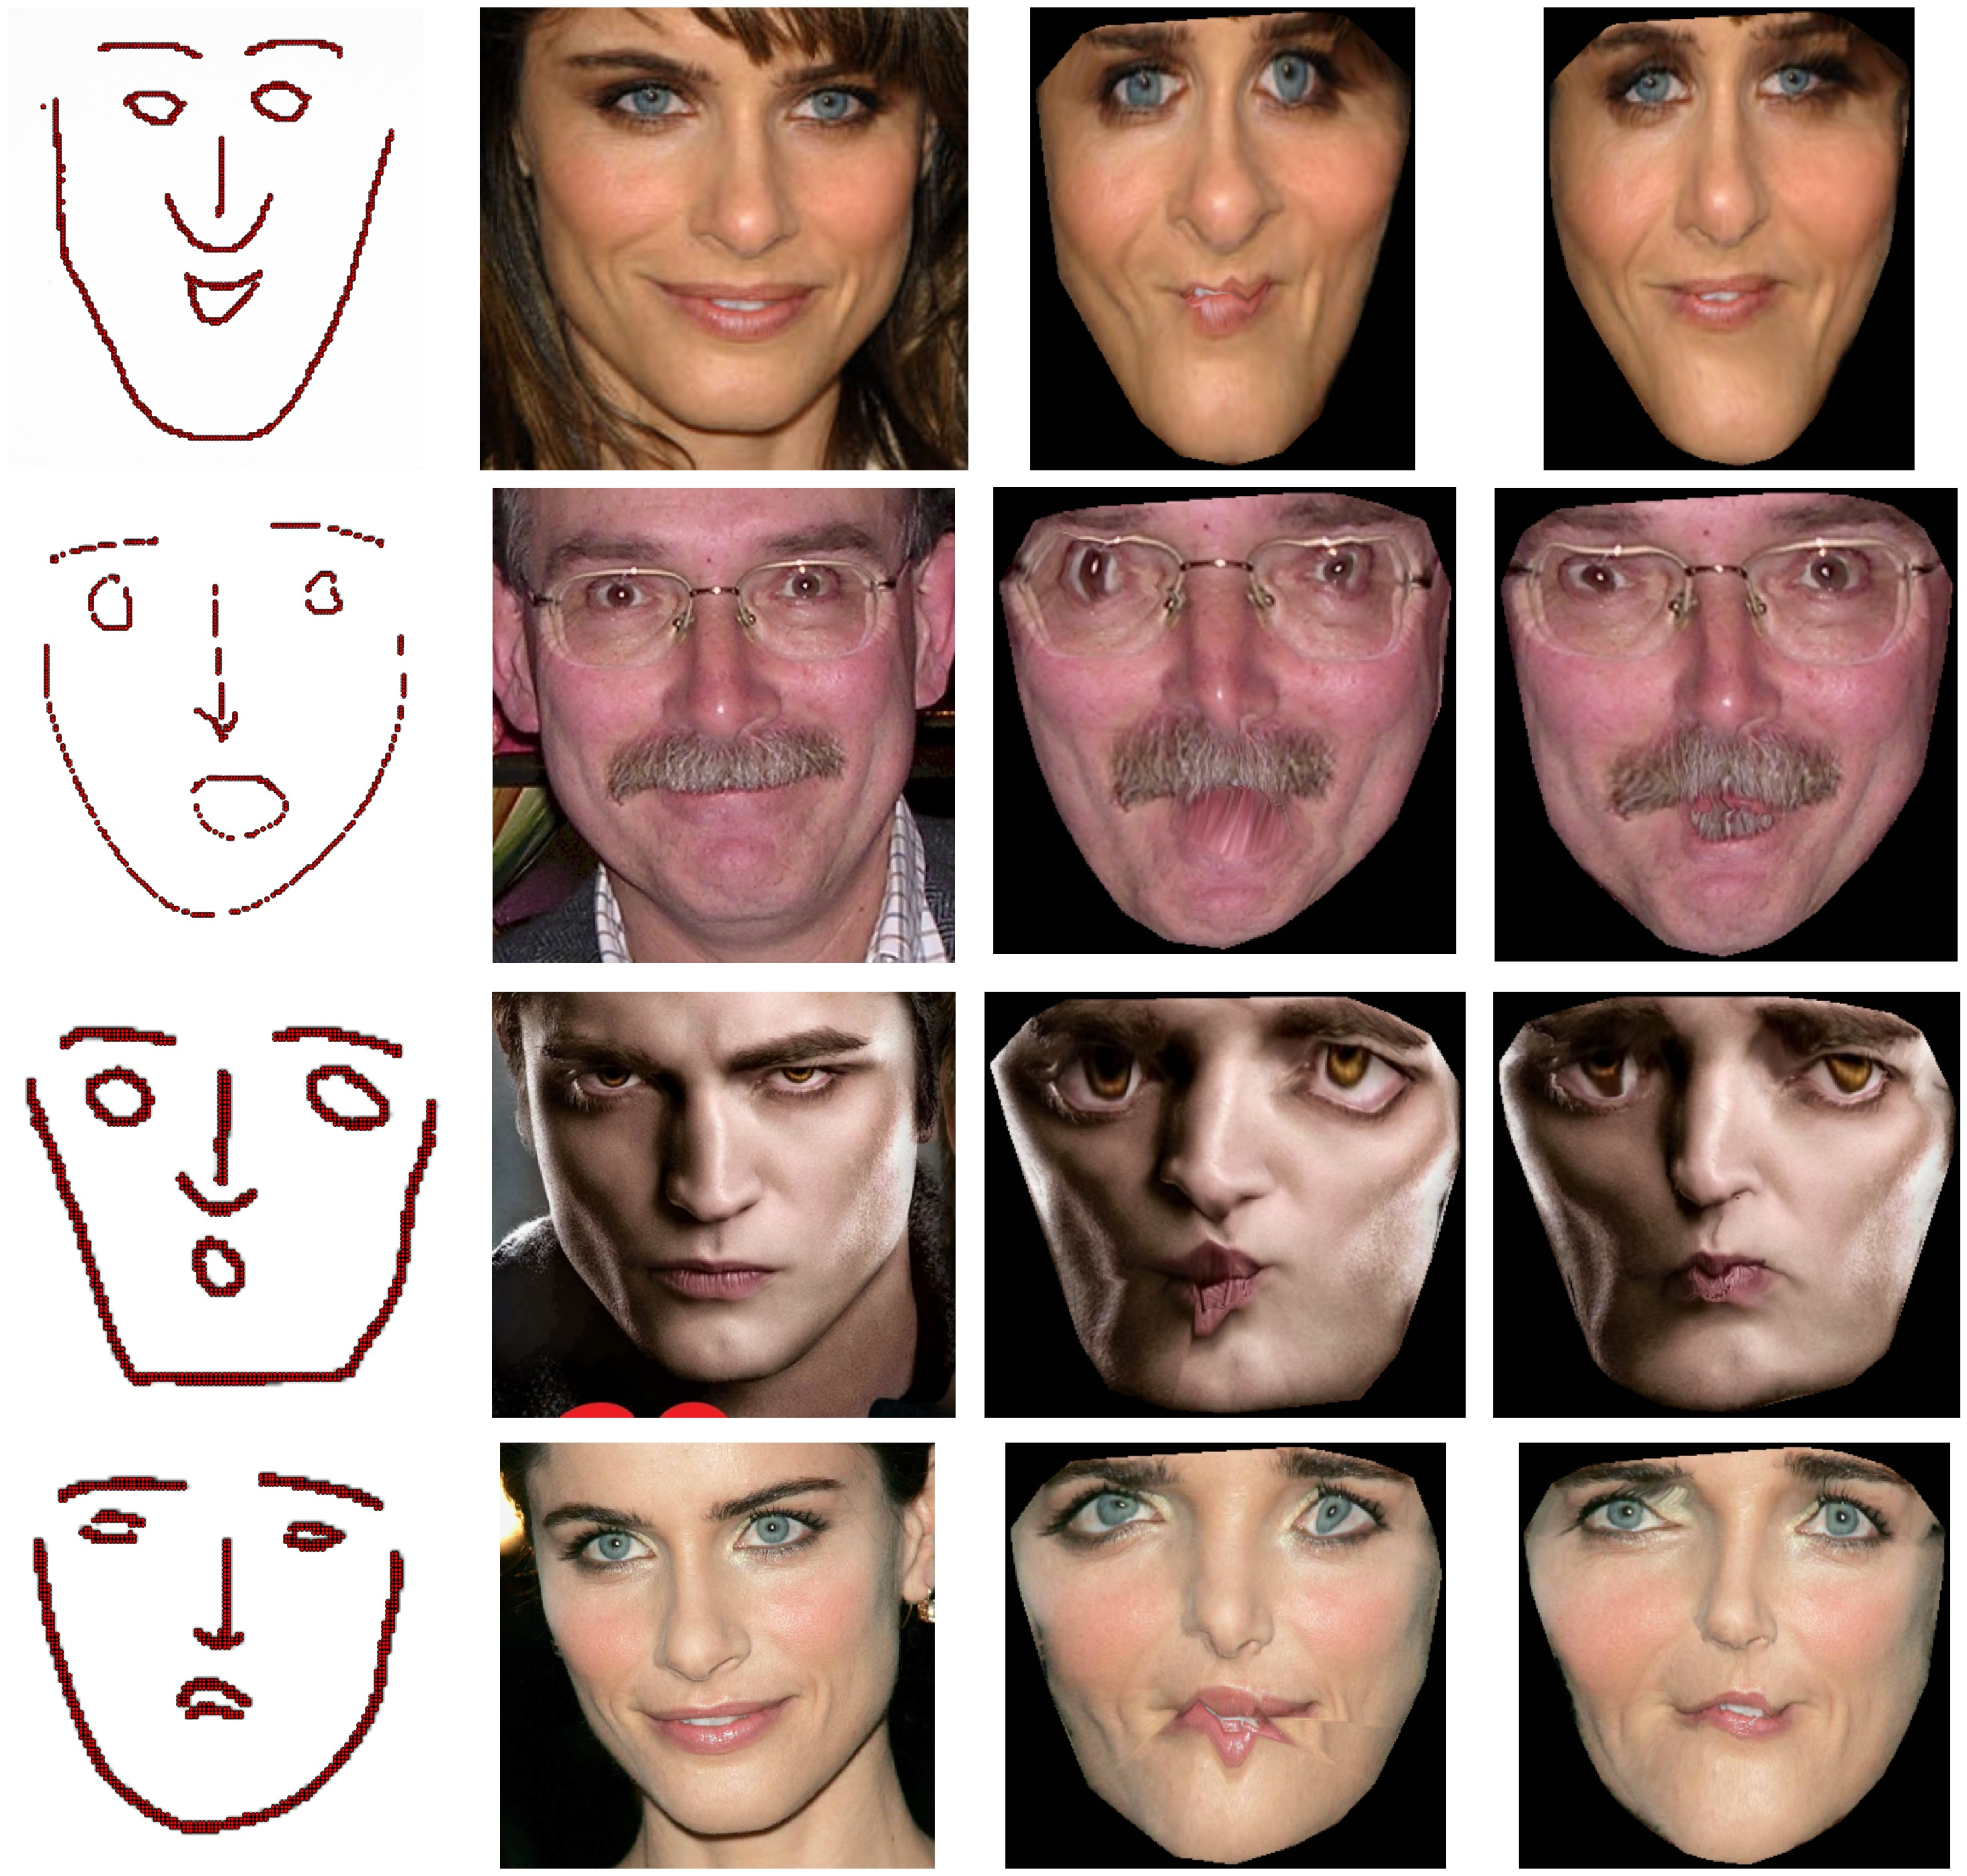
\includegraphics[width=0.45\textwidth]{resources/Fig_Draw/draw}
%    \caption{Figure}
%    \label{fig:draw}
%\end{figure}

% \clearpage

%\begin{figure}[h!]
%    \centering
%    \begin{subfigure}[b]{0.45\textwidth}
%        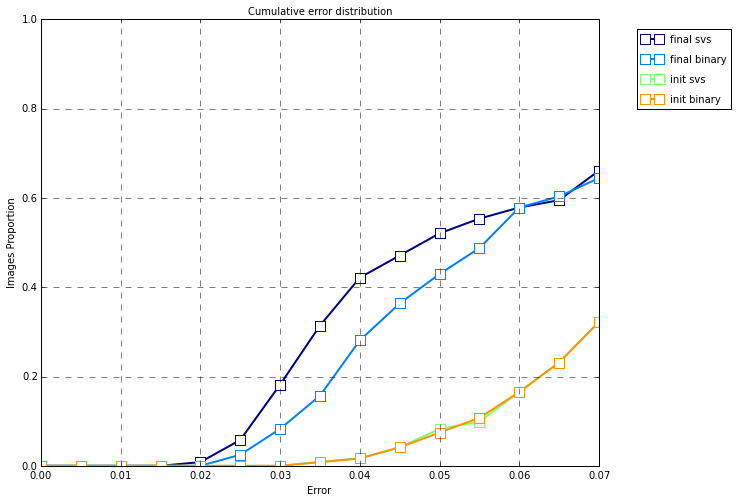
\includegraphics[width=\textwidth]{resources/Fig_SVS/faces_svs_binary_gaussian}
%        \caption{AAM Principle Components Contribution}
%    \end{subfigure}
%    \hfill
%    \begin{subfigure}[b]{0.2\textwidth}
%            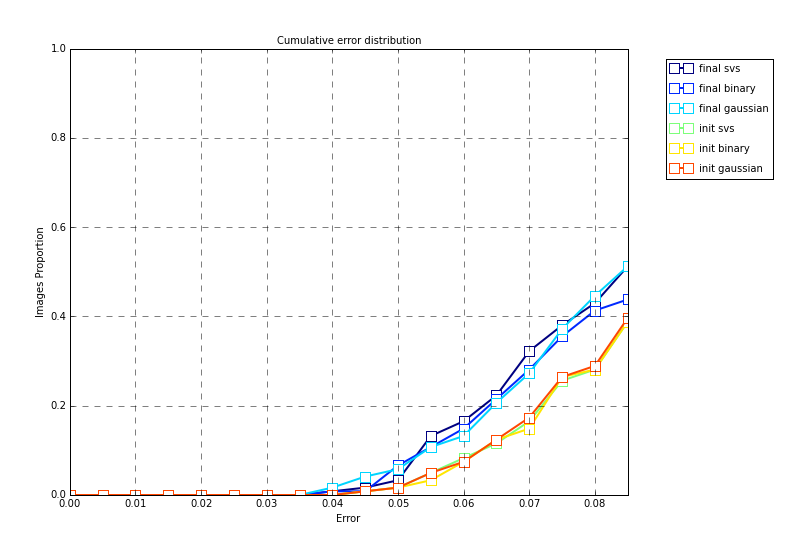
\includegraphics[width=\textwidth]{resources/Fig_SVS/ears_svs_binary_gaussian}
%        % \caption{Shape Flow Principle Components Contribution}
%    \end{subfigure}
%    \\
%    \begin{subfigure}[b]{0.2\textwidth}
%            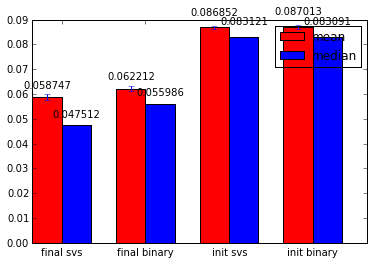
\includegraphics[width=\textwidth]{resources/Fig_SVS/faces_svs_binary_gaussian_statistics}
%        % \caption{AAM Principle Components Contribution}
%    \end{subfigure}
%    \hfill
%    \begin{subfigure}[b]{0.2\textwidth}
%            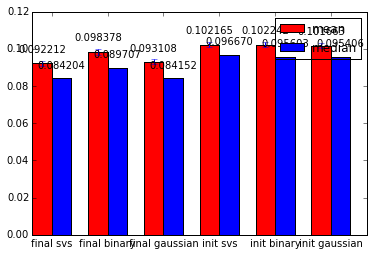
\includegraphics[width=\textwidth]{resources/Fig_SVS/ears_svs_binary_gaussian_statistics}
%        % \caption{Shape Flow Principle Components Contribution}
%    \end{subfigure}
%    \caption{Principle Components Contribution}
%\end{figure}


%\begin{figure}[h!]
%    \centering
%    \begin{subfigure}[b]{0.2\textwidth}
%            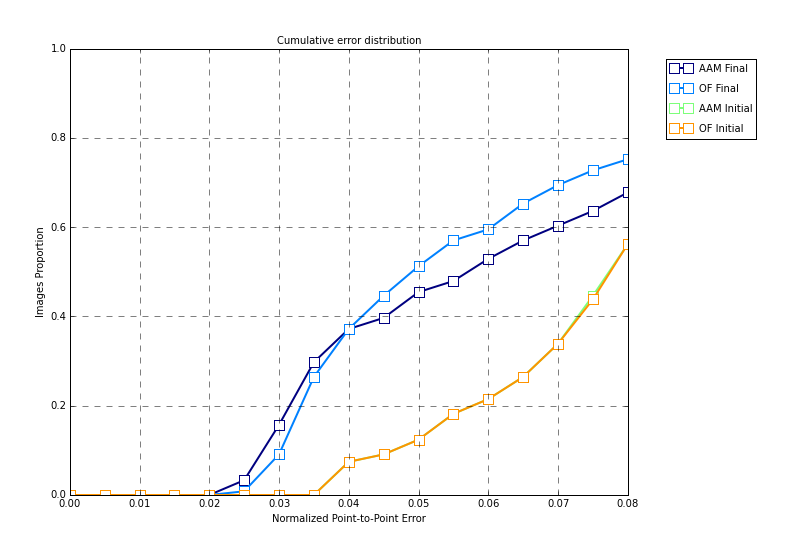
\includegraphics[width=\textwidth]{resources/Fig_Alignment/face_intensity}
%        % \caption{AAM Principle Components Contribution}
%    \end{subfigure}
%    \hfill
%    \begin{subfigure}[b]{0.2\textwidth}
%            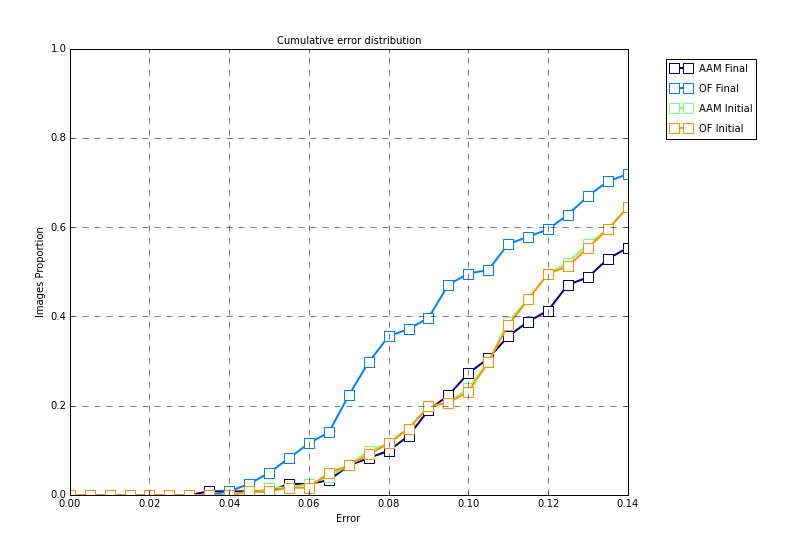
\includegraphics[width=\textwidth]{resources/Fig_Alignment/ear_intensity}
%        % \caption{Shape Flow Principle Components Contribution}
%    \end{subfigure}
%    \\
%    \begin{subfigure}[b]{0.2\textwidth}
%            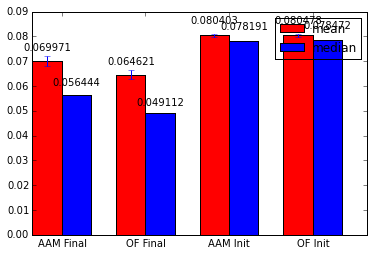
\includegraphics[width=\textwidth]{resources/Fig_Alignment/face_intensity_statistics}
%        % \caption{AAM Principle Components Contribution}
%    \end{subfigure}
%    \hfill
%    \begin{subfigure}[b]{0.2\textwidth}
%            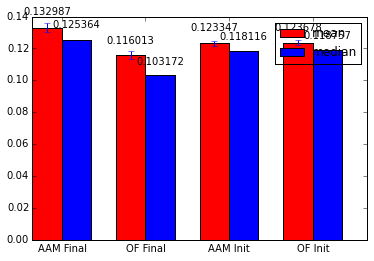
\includegraphics[width=\textwidth]{resources/Fig_Alignment/ear_intensity_statistics}
%        % \caption{Shape Flow Principle Components Contribution}
%    \end{subfigure}
%    \caption{CED Plot and Statistics of Comparison with Classic AAM}
%\end{figure}

\section{Fitting Results}
\label{sec:fittingresults}

This section provides additional visualisations for the experiments of Section 3.3 of the main submission (Non-rigid object alignment in-the-wild). We visualise pixel-wise dense fitting results for both faces and ears. Results for this experiment of faces are reported over the 224 testing images of the LFPW database using 68 point ground truth landmark annotations\footnoteref{ibug_300}. 
For ears, we collected 605 high resolution images of ears in unconstrained scenarios and annotated them using both a newly defined 55 point annotation scheme for ears and the curve annotations proposed in the report. Results for fitting ears are reported over 105 testing images.

Figure \ref{fig:fr} shows dense fitting results using a grid visualisation, thus dense points are visible without affecting the visibility of appearance.

\begin{figure}[h]
\centering
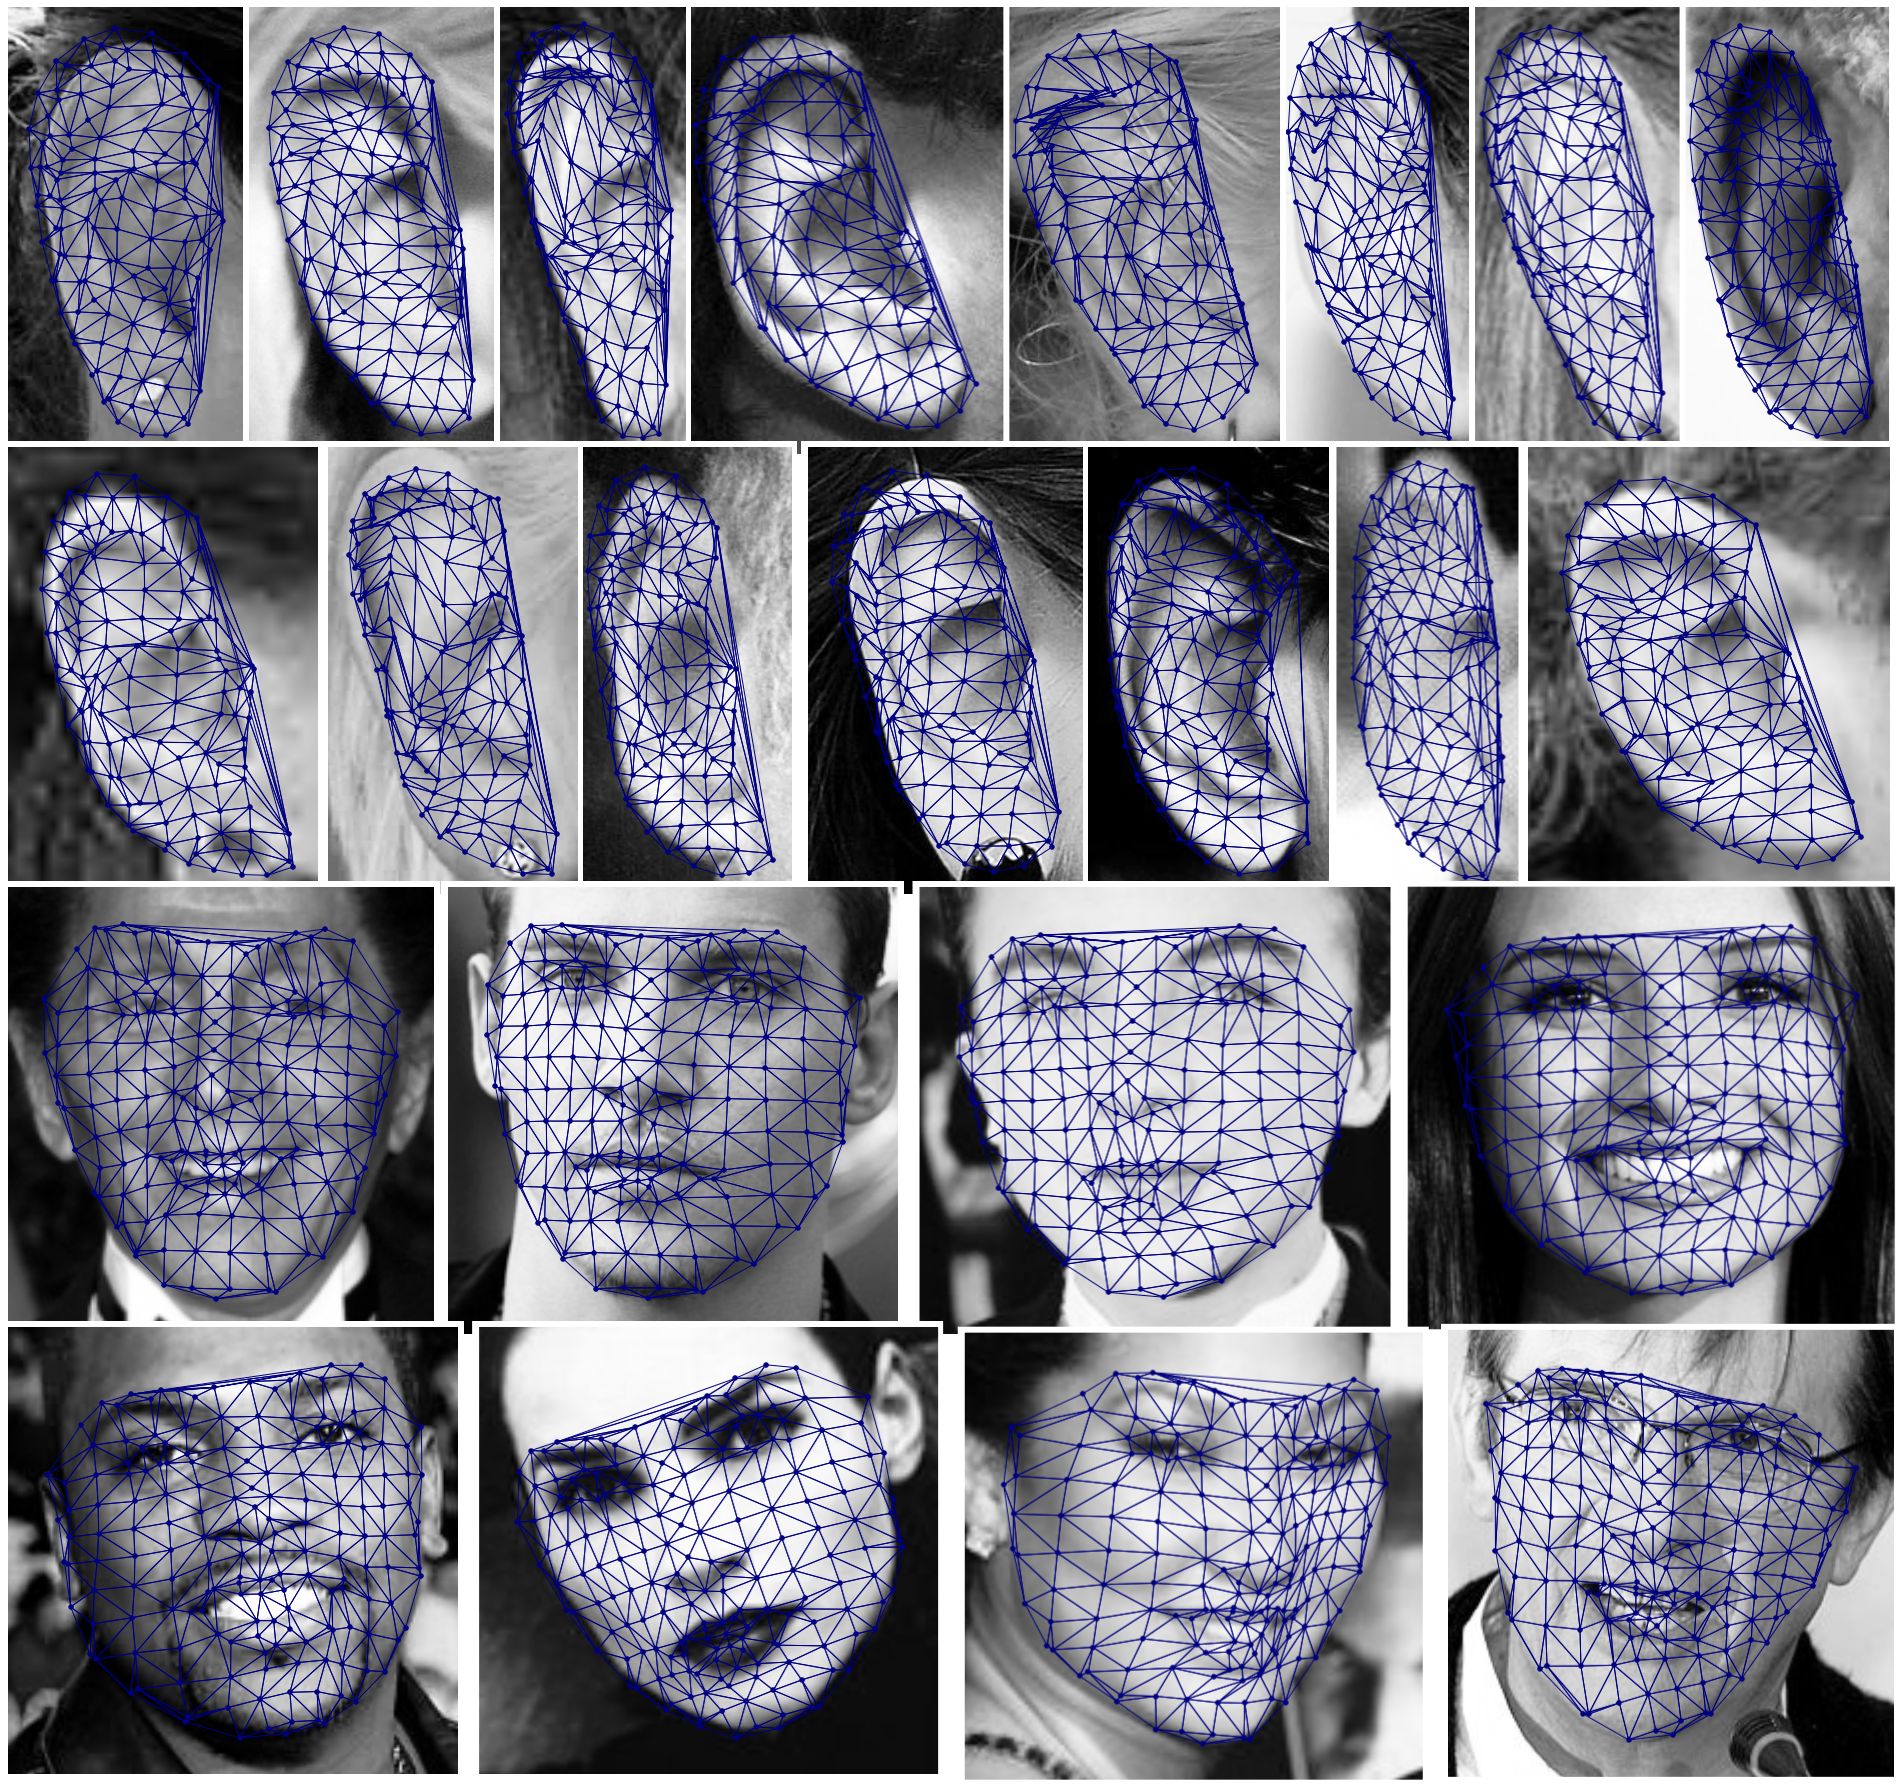
\includegraphics[width=0.6\textwidth]{supports/Fittings/fittings}
\caption{Result of fitting dAAMs on ears (first two rows) and faces (last two rows). A dense grid visualisation is used.}
\label{fig:fr}
\end{figure}


\section{Shape Model Analysis}
\label{sec:modelanalysis}

\begin{figure}[h]
    \centering
    % \vspace*{-0.1in}
    \begin{subfigure}[b]{0.45\textwidth}
            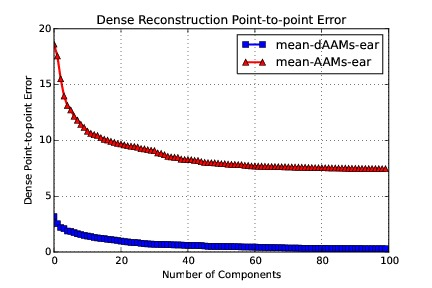
\includegraphics[width=\textwidth]{supports/Model_Analysis/sr_ear}
        %\caption{dAAMs dense shape reconstruction}
    \end{subfigure}
    \hfill
    \begin{subfigure}[b]{0.45\textwidth}
            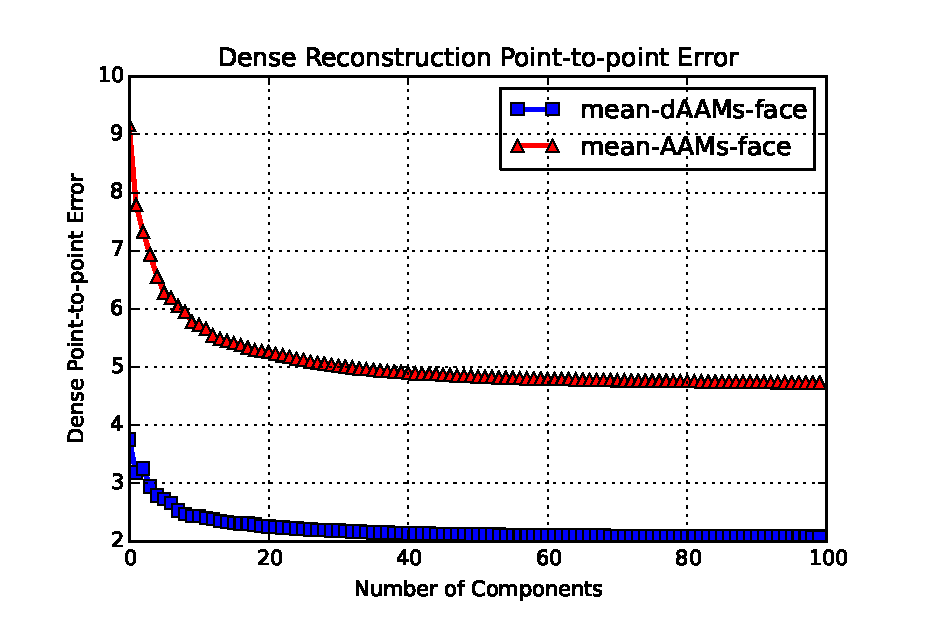
\includegraphics[width=\textwidth]{supports/Model_Analysis/sr_face}
        %\caption{AAMs dense shape reconstruction}
    \end{subfigure}
    \caption{Dense shape reconstruction errors for ears and faces. Top: results of reconstruction on ears, bottom: results of reconstruction on faces. The normalised point-to-point error is used an evaluation measure.}
    \label{fig:rc_face}
\end{figure}


We first investigate the reconstruction accuracy of AAMs and dAAMs in the shape space. In particular, given a ground-truth shape, we use the shape models from both AAMs and dAAMs to reconstruct the given shape densely. Since AAMs contain a sparse shape model, we densify it using a piecewise affine transformation, which is typically used in warping textures on to shape model too. Figure \ref{fig:rc_face} shows plots of dense shape reconstruction errors for ears and faces, for varying number of principal components kept. We observe that dAAMs significantly outperform classic AAMs on shape reconstruction. 


Furthermore, we explore the compactness of the built AAMs and dAAMs models. 
Figure \ref{fig:compact} demonstrates the variance explained as a function of the number of principal components. One can infer that dAAMs have a more compact shape model than AAMs, which leads to better reconstruction especially with few shape components.

\begin{figure}[h]
    \centering
    \begin{subfigure}[b]{0.45\textwidth}
            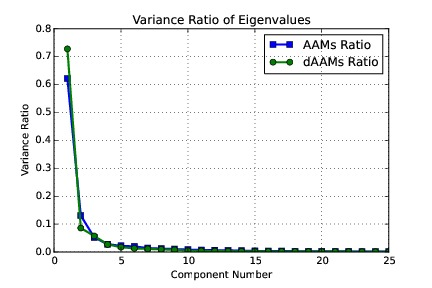
\includegraphics[width=\textwidth]{supports/Model_Analysis/var_ratio}
        %\caption{dAAMs vs AAMs Variance Ratio}
    \end{subfigure}
    \hfill
    \begin{subfigure}[b]{0.45\textwidth}
            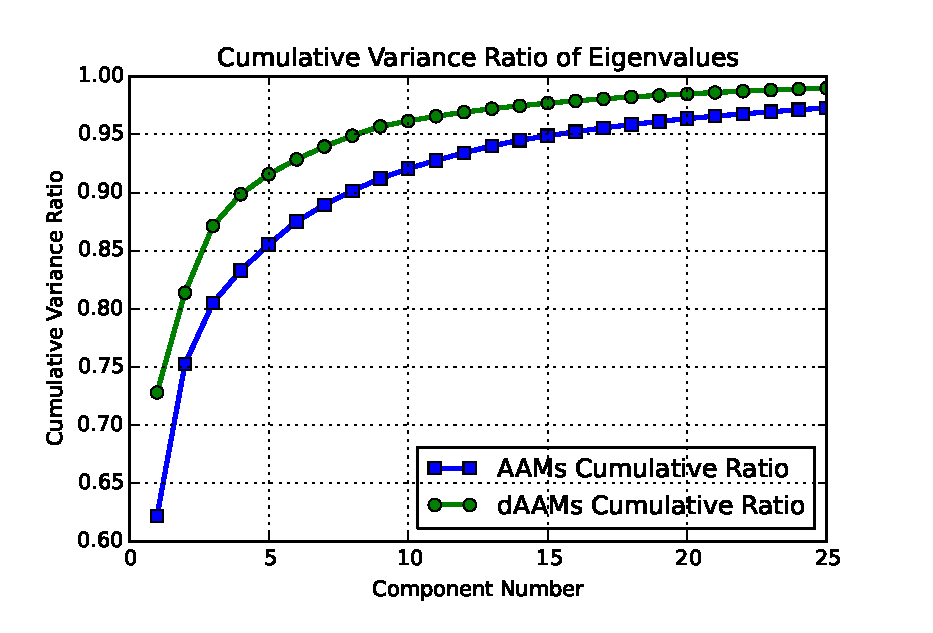
\includegraphics[width=\textwidth]{supports/Model_Analysis/cumu_var_ratio}
        %\caption{dAAMs vs AAMs Cumulative Variance Ratio}
    \end{subfigure}
    \caption{Variance explained by each principal component, for both dAAM and AAM models. Top: variance explained by each principal component. Bottom: cumulative plot of the variance explained as a function of the principal components.}
    \label{fig:compact}
\end{figure}

Finally, Figure \ref{fig:pcamodel} visualises the principal components of dAAMs for ears and faces. We observe that the variation of both shape and appearance captured by the model seem plausible.

\begin{figure*}[h]
\centering
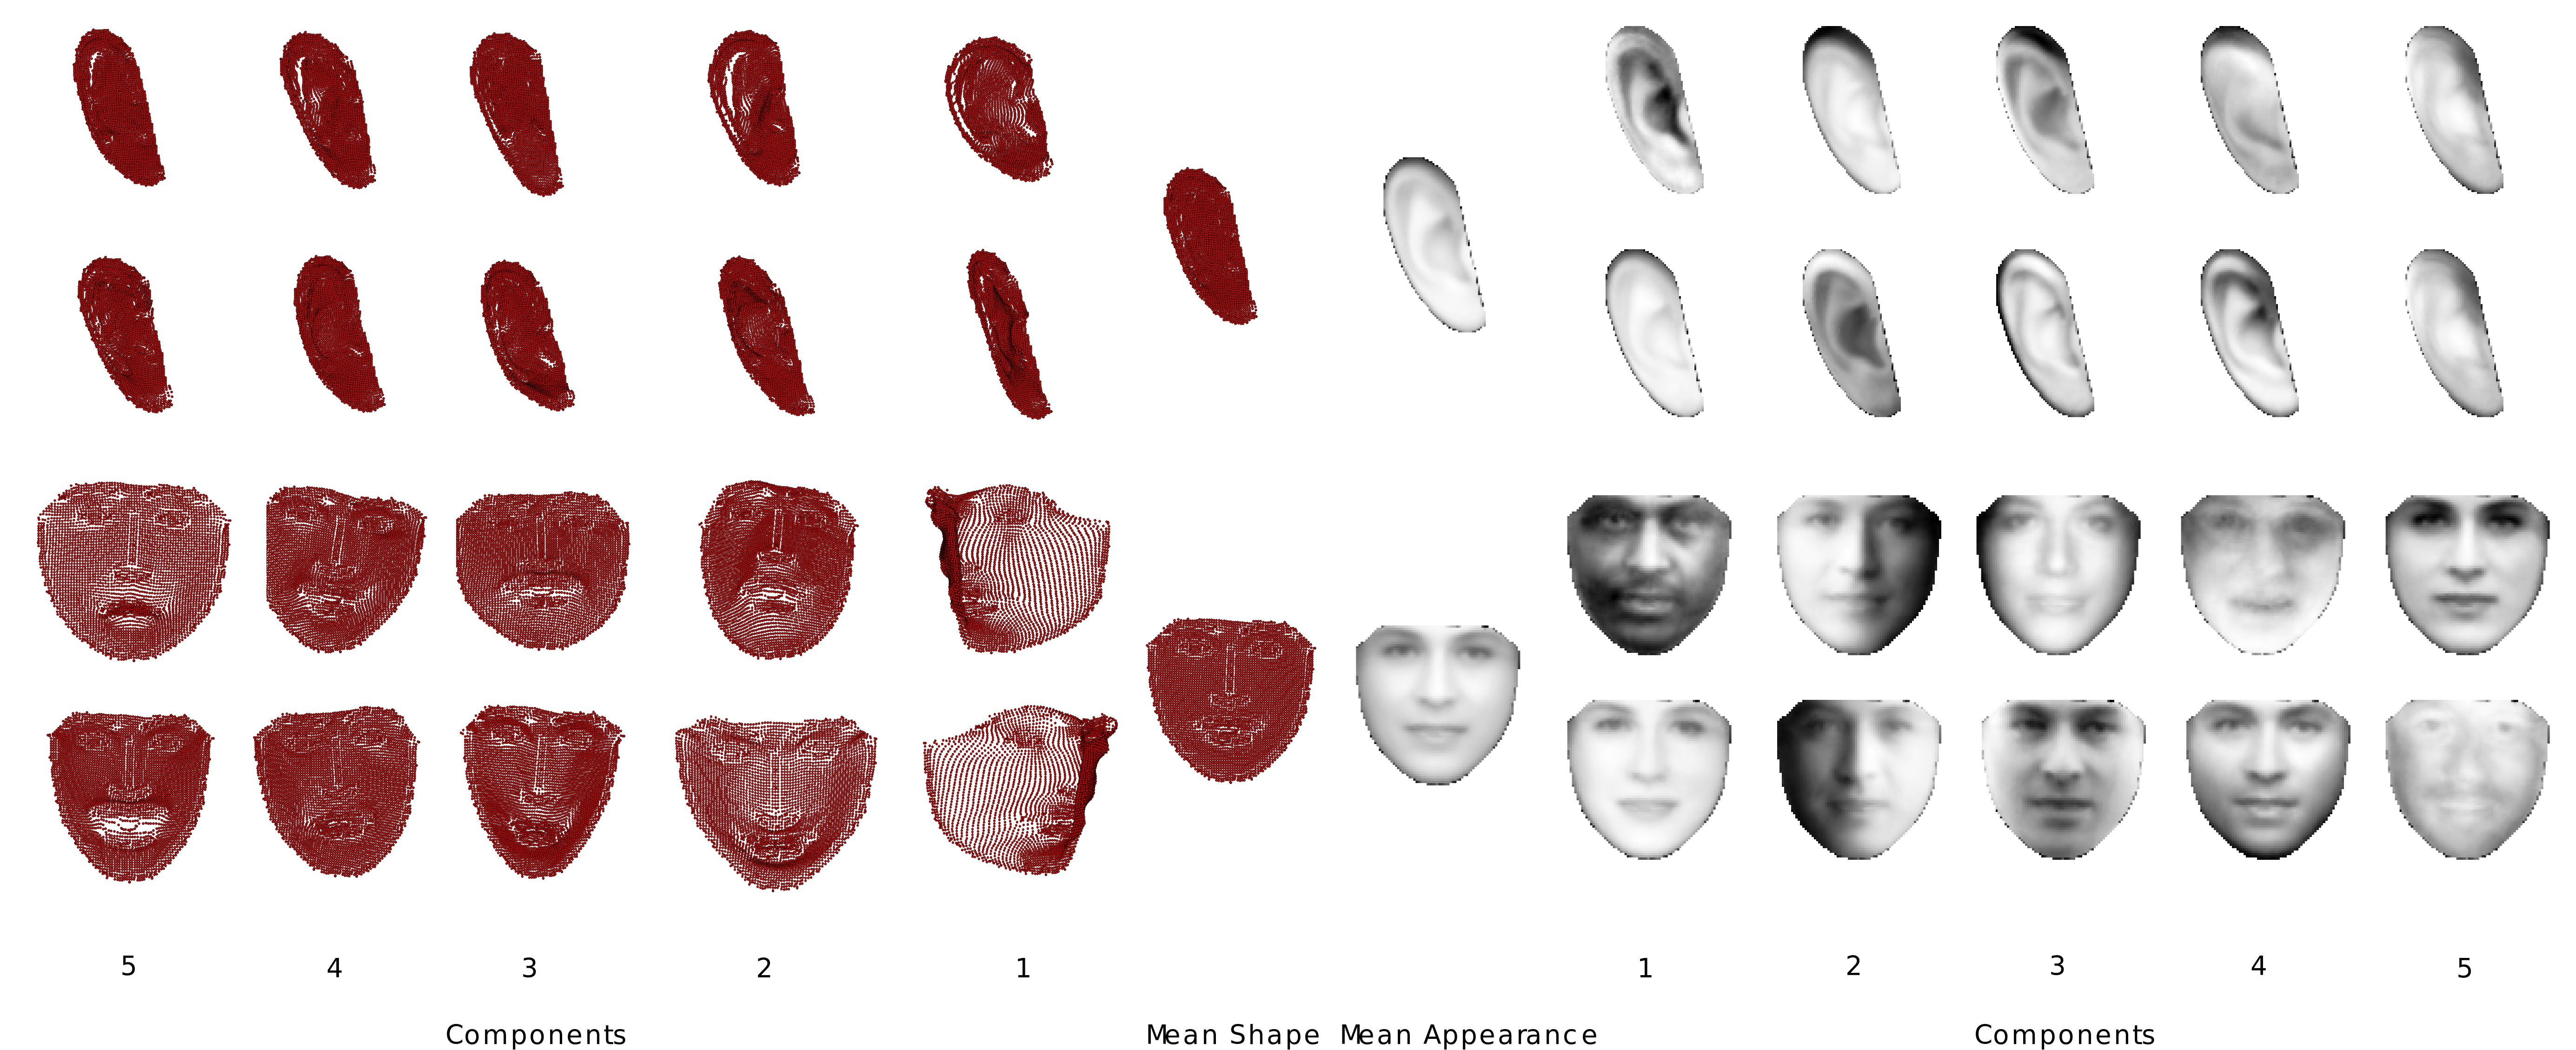
\includegraphics[width=\textwidth]{supports/Models/models}
\caption{Principal components of dAAMs built on ears (top) and faces (bottom). The mean (middle columns) as well as the first five principal components are visualised for both shape (left) and appearance (right). $\pm 3$ times the variance of the corresponding component is used in each case.}
\label{fig:pcamodel}
\end{figure*}




\section{Appearance Reconstruction}
\label{sec:reconstruct}

\begin{figure}[h]
    \centering
    %\vspace*{-0.2in}
    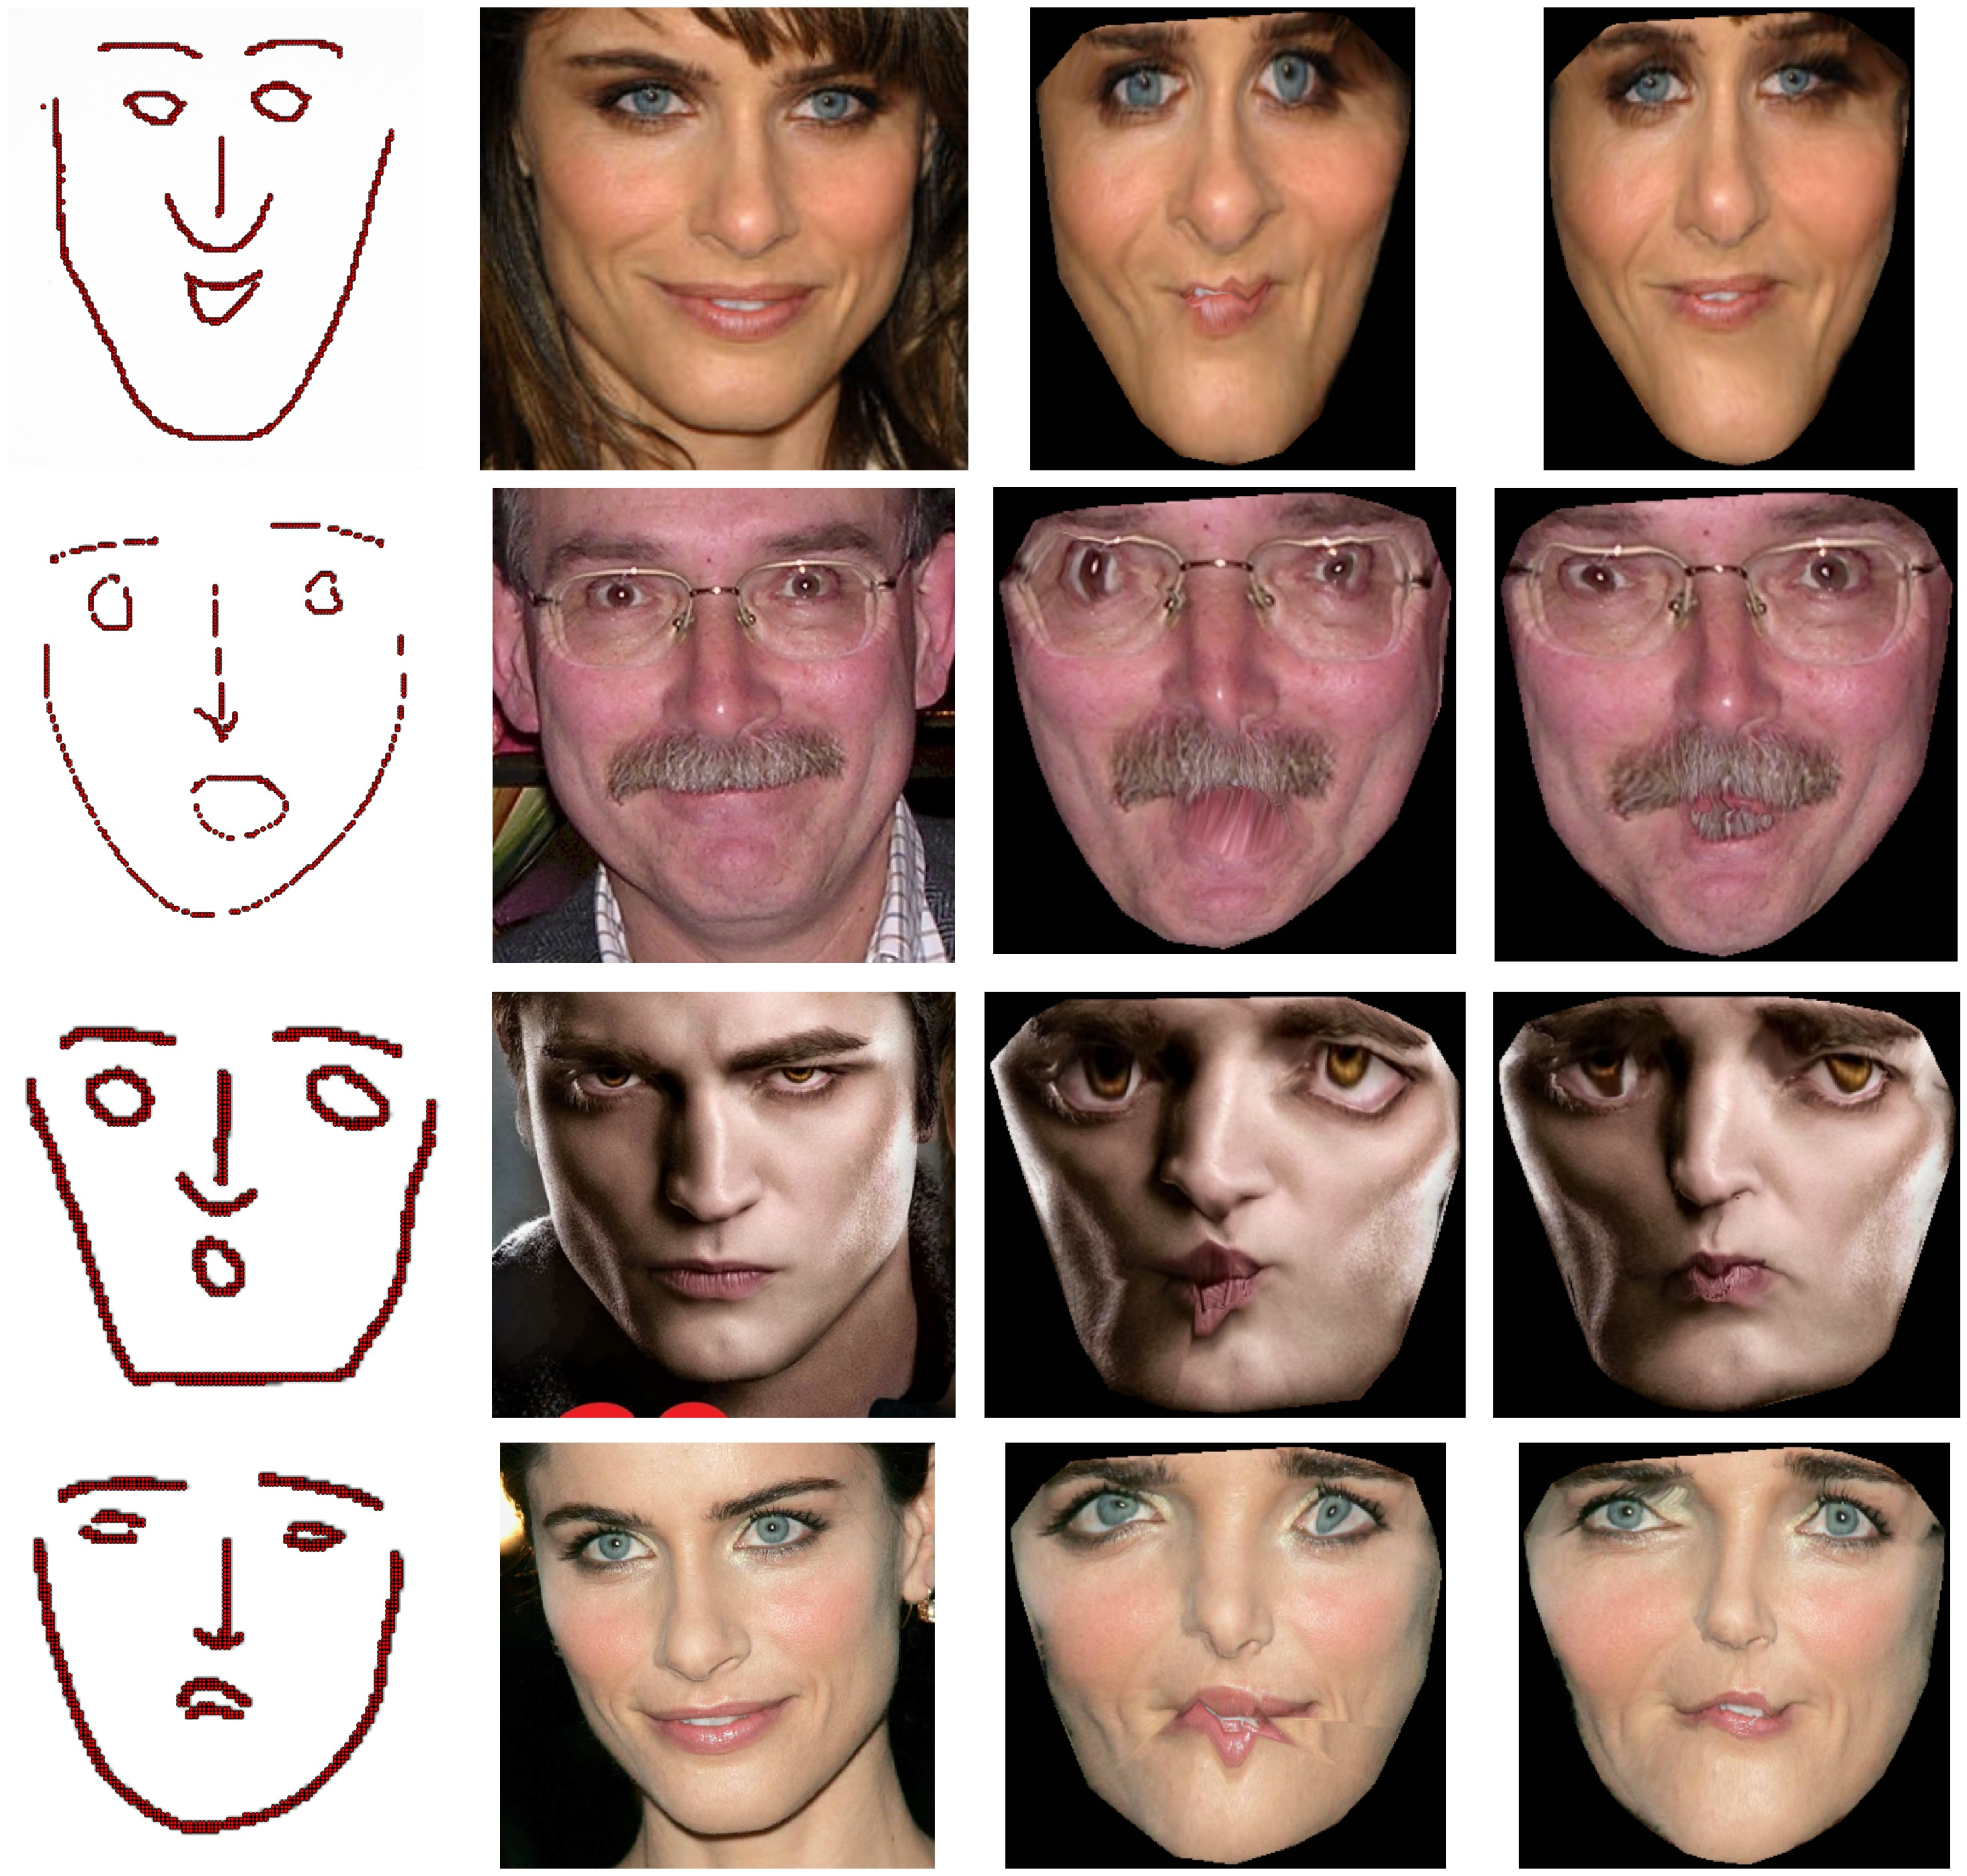
\includegraphics[width=0.6\textwidth]{resources/Fig_Draw/draw}
    \caption{Synthesizing face images from caricature sketches. First column: caricature sketches. Second column: arbitrary chosen face images. Third and last column: sketch-based warping of images based on AAMs (third column) and dAAMs (last column).}
    \label{fig:draw}
\end{figure}

In this qualitative experiment, we show how the proposed pipeline can be used to generate novel modified instances of an object, e.g. caricatures. To be specific, firstly we manually craft a set of hand-drawn cartoon-like shape sketches. We then apply shape flow to align them with the reference frame. In this way, we establish dense correspondences of landmarks. Afterwards, we perform shape reconstruction using both AAMs and dAAMs. Finally, we warp the appearance from arbitrarily chosen faces on the reconstructed shape using either piecewise affine warp (in the case of AAMs) or shape flow (in the case of dAAMs). The corresponding results are shown in figure \ref{fig:draw}. We see that AAMs introduce more severe artifacts, especially on the areas of mouth and eyes, where nuanced information is missing or models are overly deformed. In contrast, dAAMs yield a significantly more plausible result.



\section{Segmentation using Dense AAM}
\label{sec:segmentation}

In this section, we present experiments of utilising our dense AAM for object segmentation. Two object classes, bottles and human bodies, are considered. For human bodies, we use images along with ground truth segmentation from Space-Time Actions dataset \footnote{\label{sta} \url{http://www.wisdom.weizmann.ac.il/~vision/SpaceTimeActions.html}}, which includes sequences with several human actions. We use ``jumping'' and ``sliding'' actions. As far as bottles are concerned, we use 500 high-resolution images that we collected and annotated using a newly-defined 50 point annotation scheme, as well as the curve annotations proposed in this report. We randomly split these images into two disjoint sets of training (400) and testing (100) images. Bottle models were built using 400 training images while body models are built in terms of human actions (e.g. jumping), each having approximately 200 training images and 50 test images. 

\begin{figure}[h]
    \centering
    \begin{subfigure}[b]{0.3\textwidth}
            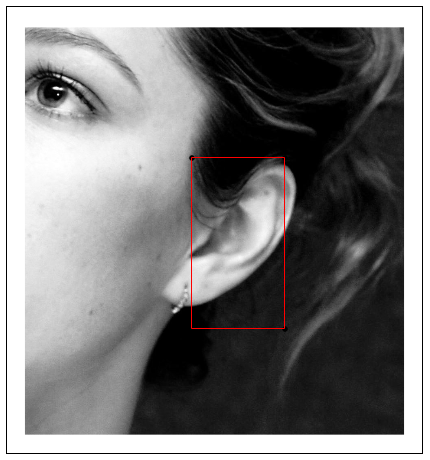
\includegraphics[height=\textwidth]{supports/Segmentation_Measure/ear}
        %\caption{Ear Initial Bounding Box}
    \end{subfigure}
    \hfill
    \begin{subfigure}[b]{0.3\textwidth}
            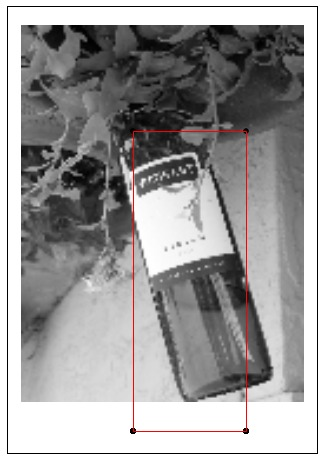
\includegraphics[height=\textwidth]{supports/Segmentation_Measure/bottle}
        %\caption{Bottle Initial Bounding Box}
    \end{subfigure}
    \hfill
    \begin{subfigure}[b]{0.3\textwidth}
            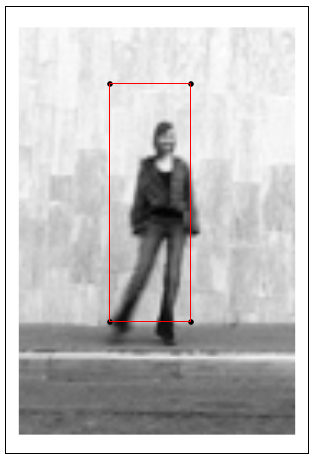
\includegraphics[height=\textwidth]{supports/Segmentation_Measure/body}
        %\caption{Body Initial Bounding Box}
    \end{subfigure}
    \caption{Examples of fitting initialisations used for the segmentation experiment. These are created by random perturbation of the ground-truth bounding box.}
    \label{fig:seg_init}
\end{figure}

Fitting dAAMs on test images yields dense landmarks that can be used to perform segmentation. In a real-world scenario, a simple object detector would be required to be applied prior to our pipeline to initialise the fitting. However, as a simple evaluation, we initialise the fitting by randomly perturbing the ground-truth bounding box with certain variance to simulate an object detector with implicit detection, see e.g.~Figure \ref{fig:seg_init}. Table  \ref{tab:seg_result} reports the segmentation precision, in case of fitting bottles and human bodies by adopting the proposed dAAMs pipeline.

\begin{table}[!h]
\small
\centering
\begin{tabular}{|l|c|c|c|}
\hline
\emph{Object}   & \emph{mean} & \emph{std} & \emph{median}\\
\hline\hline
Bottles         & 0.8125      & 0.1460     & 0.8414\\
Action - Jump   & 0.6102      & 0.0198     & 0.6099\\
Action - Slide  & 0.6444      & 0.0500     & 0.6501\\
\hline
\end{tabular}
\caption{Segmentation precision, in case of fitting bottles and human bodies by adopting the proposed dAAMs pipeline. The mean, standard deviation and median of the precision error are provided.}
\label{tab:seg_result}
\end{table}